\documentclass[11pt]{article}
\usepackage{amsmath,amssymb,amsthm,booktabs,hyperref,graphicx}
% Portable Type1 font settings; no additional packages are loaded.
\renewcommand{\encodingdefault}{T1}
\DeclareFontFamily{T1}{paperroman}{}
\DeclareFontShape{T1}{paperroman}{m}{n}{<-> ec-lmr10}{}
\DeclareFontShape{T1}{paperroman}{m}{it}{<-> ec-lmri10}{}
\DeclareFontShape{T1}{paperroman}{m}{sc}{<-> ec-lmcsc10}{}
\DeclareFontShape{T1}{paperroman}{bx}{n}{<-> ec-lmbx10}{}
\DeclareFontShape{T1}{paperroman}{b}{n}{<-> ssub * paperroman/bx/n}{}
\DeclareFontFamily{OT1}{paperoperators}{}
\DeclareFontShape{OT1}{paperoperators}{m}{n}{<-> rm-lmr10}{}
\DeclareFontShape{OT1}{paperoperators}{bx}{n}{<-> rm-lmbx10}{}
\DeclareFontFamily{T1}{papermono}{}
\DeclareFontShape{T1}{papermono}{m}{n}{<-> ec-lmtt10}{}
\DeclareFontFamily{OML}{paperletters}{}
\DeclareFontShape{OML}{paperletters}{m}{it}{<-> lmmi10}{}
\DeclareFontFamily{OMS}{papersymbols}{}
\DeclareFontShape{OMS}{papersymbols}{m}{n}{<-> lmsy10}{}
\DeclareFontFamily{OMX}{paperlarge}{}
\DeclareFontShape{OMX}{paperlarge}{m}{n}{<-> lmex10}{}
\renewcommand{\rmdefault}{paperroman}
\renewcommand{\sfdefault}{paperroman}
\renewcommand{\ttdefault}{papermono}
\SetSymbolFont{operators}{normal}{OT1}{paperoperators}{m}{n}
\SetSymbolFont{letters}{normal}{OML}{paperletters}{m}{it}
\SetSymbolFont{symbols}{normal}{OMS}{papersymbols}{m}{n}
\SetSymbolFont{largesymbols}{normal}{OMX}{paperlarge}{m}{n}
\SetMathAlphabet{\mathbf}{normal}{OT1}{paperoperators}{bx}{n}
\SetMathAlphabet{\mathit}{normal}{T1}{paperroman}{m}{it}
\SetMathAlphabet{\mathtt}{normal}{T1}{papermono}{m}{n}
% Permit line breaks in long formal identifiers and bibliography URLs.
\makeatletter
\g@addto@macro\UrlBreaks{\do\a\do\b\do\c\do\d\do\e\do\f\do\g\do\h\do\i\do\j\do\k\do\l\do\m\do\n\do\o\do\p\do\q\do\r\do\s\do\t\do\u\do\v\do\w\do\x\do\y\do\z\do\A\do\B\do\C\do\D\do\E\do\F\do\G\do\H\do\I\do\J\do\K\do\L\do\M\do\N\do\O\do\P\do\Q\do\R\do\S\do\T\do\U\do\V\do\W\do\X\do\Y\do\Z\do\_}
\makeatother

\hypersetup{hidelinks,pdftitle={Obstructions and Formalized Identities in Two Binary Goldbach Research Programmes},pdfauthor={Durand Serge},pdfsubject={Negative results and formalization; no assertion resolving binary Goldbach}}
\setlength{\textwidth}{16cm}
\setlength{\oddsidemargin}{0cm}
\setlength{\evensidemargin}{0cm}
\setlength{\textheight}{23cm}
\setlength{\topmargin}{-1cm}
\setlength{\emergencystretch}{3em}
\setlength{\parskip}{3pt}
\setlength{\tabcolsep}{3pt}
\renewcommand{\arraystretch}{1.12}
\newcommand{\ev}[1]{{\scriptsize[\nolinkurl{#1}]}}
\newcommand{\evidence}[1]{\ev{#1}}
\newcommand{\Lam}{\Lambda}
\newcommand{\Q}{\mathbb{Q}}
\newcommand{\F}{\mathbb{F}}
\newcommand{\N}{\mathbb{N}}
\newcommand{\C}{\mathbb{C}}
\newcommand{\R}{\mathbb{R}}
\newcommand{\Z}{\mathbb{Z}}
\newcommand{\status}[1]{\textbf{#1}}
\newtheorem{theorem}{Theorem}[section]
\newtheorem{proposition}[theorem]{Proposition}
\newtheorem{definition}[theorem]{Definition}
\theoremstyle{remark}
\newtheorem{remark}[theorem]{Remark}
\title{Obstructions and Formalized Identities\\in Two Binary Goldbach Research Programmes\\[4pt]\large A Negative-Results and Formalization Report}
\author{Durand Serge\\\small Independent researcher\\\small\texttt{seisner1967@gmail.com}}
\date{5 October 2026}
\begin{document}
\maketitle
\begin{abstract}
We record obstructions and established formalizations in an analytic corpus and
an algebraic certificate campaign concerning binary Goldbach. The analytic
results include exact coefficient projection, finite character extraction,
canonical logarithm quantization, finite-field roots, and credited portions of
the Mellin inversion dependency chain. Their scope is separated from
uncompiled truncation sources and from the signed estimate still required for
a prime-pair lower bound. The algebraic results include ordinary-polynomial
soundness, calibration, uniform common-zero constructions for specified
constraint families, and a rational static Nullstellensatz degree lower bound.
Finite measurements attain that bound at the measured points; a universal
matching construction is not established. Polynomial-calculus measurements
and its explicitly assumed external lower-bound predicate are kept distinct.
A completed integer and CRT computation at a single finite input is reported
without a Lean refinement claim. An evidence map and generated Lean inventory
identify the supporting artifacts and their exact verification levels. The
report establishes no conclusion resolving binary Goldbach and excludes
neither the full analytic programme nor the full algebraic certificate route.
\end{abstract}
\noindent\textbf{MSC2020:} 11P32 (primary); 68V20, 03F20, 13P10 (secondary).\ev{R-MSC}
\par\noindent\textbf{Suggested arXiv classification:} math.NT; possible cross-lists
cs.LO and cs.CC, subject to the author's submission decision.

\section{Introduction and scope}
Binary Goldbach asks whether every even integer greater than two is the sum
of two primes.\ev{R-FROZEN} The distinction between a useful identity and a sufficient
prime-pair lower bound is central to this report. The classical context
includes the Hardy--Littlewood formulation, Vinogradov's three-prime theorem,
Chen's prime and almost-prime theorem, and the ternary theorem of
Helfgott.\cite{hl1923,vinogradov1937,chen1973,helfgott2013}
The published finite verification up to $4\cdot10^{18}$ is a different kind
of evidence from a theorem covering all even integers.\cite{osilva2014}

We consolidate the round-22 analytic corpus as summarized in Synthesis V3.1
and the stopped AlgebraicGoldbach campaign.\ev{R-CORPORA}
Existing material from the historical Horizon repository is admitted only
where an existing Judge record supplies the stated credit; a source file or
a project README alone is insufficient. No new mathematical execution was
performed for this manuscript.\ev{R-STOP}
Classical projection, Mellin inversion and finite counting arguments are
recorded or formalized here without claims of novelty. Literature on
Nullstellensatz and polynomial calculus supplies context, rather than a
replacement for the hypotheses of the project statements.
\cite{ips1997,cei1996,bikpp1996,razborov1998,alon1999}

\noindent\textbf{How to read this report.}
\par First read the evidence label attached to a result.
\par Then read its domain, hypotheses and mathematical object.
\par Finally consult its evidence key in the machine-readable map and the
inventory before treating a source or finite observation as a theorem.

\section{Evidence levels and verification protocol}
\begin{center}\small
\begin{tabular}{p{2.3cm}p{12.6cm}}
\toprule
Level & Meaning in this report\\
\midrule
Compiled Lean & An existing successful Lean record covers the declaration;
the available axiom record is reported. It does not certify a different
informal statement or remove its explicit hypotheses.\\
SOURCE & A written Lean source exists without the required successful
compile credit for that item.\\
PAPER & An existing written mathematical argument or review is recorded;
it is not promoted to compiled formal proof.\\
Observed & An existing process, file or finite measurement was recorded;
the observation is limited to that run and input.\\
EVIDENCE & Existing independently checked finite arithmetic, model or
certificate data support precisely the stated finite claim.\\
\bottomrule
\end{tabular}
\end{center}
These levels do not form an automatic implication chain. In particular,
source availability, a passing build, an axiom list and a finite certificate
answer different questions. Explicit theorem premises remain premises even
when the declaration uses only the standard logical axioms.\ev{R-PROTOCOL}

The campaign protocol used separate implementation, adversarial reading and
Judge roles, source pins, exact ordinary polynomial definitions, and
valid-data-first corruption controls. The accepted evidence identifies the
actual command and result, rather than treating an agent's summary as a
proof.\ev{R-PROTOCOL}
The paper's fresh compilation and claim-to-evidence review concern this
document only. They neither rerun the mathematical experiments nor add
Judge credit to their results.\ev{R-STOP}

\subsection{Limitations of the verification arrangement}
The agent roles share a model provider and are not an external mathematical
referee panel. Their separation is operational; it does not imply
statistical independence or third-party validation. The Lean kernel checks
formal terms under their recorded assumptions. Interpretation of those
terms, choice of constraints, and correspondence with a native program
still require human review.\ev{R-PROTOCOL}

The preserved Windows artifacts distinguish raw bytes, Git blobs and
historical documentary snapshots. CRLF transport and path separators caused
reader and binding problems; named corrections do not justify silently
normalizing old reports. The manuscript cites the original artifact hashes
and keeps documentary transport distinct from mathematics.\ev{R-WINDOWS}
The repository already contains the LF text policy requested for this
publication; no existing file was converted for the paper.\ev{R-ATTRIBUTES}

The algebraic frozen target is a bare, unfinished theorem declaration. It
contains no proof term and is excluded from the auxiliary build. Freezing
the entire file's bytes prevents adding a proof without changing the file
hash. Thus the frozen-file rule cannot simultaneously accept a newly added
proof of that declaration. This is a design flaw in the target acceptance
contract, not a mathematical obstruction. The frozen bytes remain
unchanged.\ev{R-FROZEN}

\section{Analytic framework and the credited dependency chain}
\label{sec:analytic}

The analytic corpus supplies exact identities and explicit approximation
bounds. Its recorded Judge receipts distinguish successful module rows from
the status of an entire batch. This distinction matters for batches 6, 7, 8,
9, 11 and 26: each globally failed batch retains only the whole-module PASS
rows identified in the inventory. No failed or uninvoked module is credited.
The standard axioms recorded for credited declarations are subsets of
\texttt{propext}, \texttt{Classical.choice} and \texttt{Quot.sound}.
Appendix~\ref{app:analytic-inventory} provides a module table; the accompanying
JSON and CSV retain every extracted axiom-audit row.\ev{A-PARTIAL-BATCHES}
\ev{A-INVENTORY-COUNTS}

\subsection{The genuine coefficient and its continuous projection}

Throughout this section, $\Lambda$ is the genuine von Mangoldt function:
$\Lambda(0)=\Lambda(1)=0$, $\Lambda(p^k)=\log p$ for a prime $p$ and
an integer $k\geq1$, and it vanishes otherwise. For $a>0$, set
\begin{equation}
 T_a(\theta)=\sum_{n\geq0}\Lambda(n)e^{-an}e^{in\theta},\qquad
 C_N=\sum_{n=0}^{N}\Lambda(n)\Lambda(N-n).
 \label{eq:analytic-definitions}
\end{equation}
The series is absolutely convergent. The compiled continuous projection
identity, for every natural $N$, is
\begin{equation}
 C_N=\frac{e^{aN}}{2\pi}\int_0^{2\pi}
          T_a(\theta)^2e^{-iN\theta}\,d\theta.
 \label{eq:circle-identity}
\end{equation}
This is \nolinkurl{thermalContinuousProjection_eq_vonMangoldt_sum}
in the module \nolinkurl{ThermalProjectionIdentity22}.
The source uses the full interval $[0,2\pi]$. Prime powers remain in $C_N$;
the equality alone is not a lower bound for a prime-pair sum. The square
$T_a^2$ extracts additive pairs. Replacing it by $|T_a|^2$ extracts
differences and changes the coefficient being studied.\ev{A-CIRCLE}
\ev{A-OBSTRUCTION-SIGNED-GAP}

There is also a compiled elementary truncation envelope. With $r=e^{-a}$,
let
\begin{equation}
 U(a)=\frac{r}{(1-r)^2},\qquad
 B(a,M)=r^{M+1}\left(\frac{M+1}{1-r}+U(a)\right).
\end{equation}
If $T_{a,M}$ is the sum through $M$, the corresponding normalized
projection differs from the full projection by at most
$2e^{aN}U(a)B(a,M)$ in complex norm. The bound follows from actual
von Mangoldt terms and a constructed summable majorant, rather than from
an assumed coefficient bound. Its module is a retained PASS row in failed
batch 11.\ev{A-CIRCLE}

\subsection{Finite projection and canonical logarithm quantization}

For natural $N\leq M$ and $K>\max(N,2M-N)$, the discrete projector satisfies
\begin{equation}
 C_N=\frac{e^{aN}}{K}\sum_{j=0}^{K-1}
 T_{a,M}(2\pi j/K)^2 e^{-2\pi iNj/K}.
 \label{eq:discrete-projector}
\end{equation}
The condition excludes all unwanted exponents congruent to $N$ modulo $K$.
This is a finite identity for every real $a$, including $a=0$; it does not
assert convergence of the infinite series at $a=0$.
The declaration \nolinkurl{sampled_trueCircle_eq_coefficient}
in \nolinkurl{DiscreteThermalProjection22}
records the concrete angular grid.\ev{A-DISCRETE}

The quantized construction uses the fixed scale $S=2^{58}$. Define
\begin{equation}
 L_{32}(z)=2\sum_{j=0}^{31}\frac{z^{2j+1}}{2j+1},\qquad
 \rho_{32}=\frac{9}{4\cdot65\cdot3^{65}}.
\end{equation}
For $2\leq p\leq10^8$, write $k=\lfloor\log_2p\rfloor$ and
$z=(p-2^k)/(p+2^k)$. The rational lower endpoint is
$b_p=kL_{32}(1/3)+L_{32}(z)$, with interval width
$(k+1)\rho_{32}$. The constructor rounds the midpoint multiplied by $S$
to the nearest integer, resolving exact ties toward the even integer,
then clamps to $[0,32S]$. The proved error is at most $1/S$;
precision is a conclusion of this fixed constructor.\ev{A-LOG}

Applying the constructor to the base prime of each prime power defines
integers $A_n$ and $q_n=A_n/S$. Both $q_n$ and $\Lambda(n)$ lie in $[0,32]$
on $0\leq n\leq10^8$, and $|q_n-\Lambda(n)|\leq1/S$ there. Thus, for
natural $N\leq10^8$, the canonical integer coefficient
$I_N=\sum_{n=0}^N A_nA_{N-n}$ satisfies
\begin{equation}
 \left|C_N-\frac{I_N}{S^2}\right|
 \leq E_{\log}(N):=(N+1)\left(\frac{64}{S}+\frac1{S^2}\right).
 \label{eq:log-envelope}
\end{equation}
The fixed integer guard proves $2E_{\log}(10^8)\leq10^{-6}$.
These statements are in \nolinkurl{RationalLogQuantization22} and
\nolinkurl{QuantizedLambdaEnvelope22}; no real-logarithm precision
assumption is inserted.\ev{A-LOG}

\subsection{Finite-field extraction and the five concrete roots}

The generic finite-field module derives character orthogonality from an
actual primitive root, then instantiates the coefficient projector for the
canonical integer sequence. The concrete root module proves the primality
of the five moduli and exact order $K=2^{27}$ of the roots
$\omega=g^{(p-1)/K}$ in their respective fields. Here $g$ denotes the
specified bank base; the needed assertion is the order of $\omega$.
\ev{A-FIELD}

\begin{center}
\begin{tabular}{rr}
\toprule Certified prime $p$ & Bank base $g$\\\midrule
2013265921 & 31\\
2281701377 & 3\\
3221225473 & 5\\
3489660929 & 3\\
3892314113 & 3\\
\bottomrule
\end{tabular}
\end{center}

At $N=M=10^8$, each such field projector returns $I_N$ modulo $p$.
The compiled results are in \nolinkurl{FiniteFieldProjection22},
\nolinkurl{ConcreteNTTRoots22} and
\nolinkurl{ConcreteNTTA32Projection22}. A theorem about this finite
projector does not by itself refine the native transform or CRT program.
The saved numerical computation is reported separately in
Section~\ref{sec:numerical}.\ev{A-FIELD}

\subsection{The actual Gamma inversion dependency chain}

The inversion chain is a sequence of credited source modules with explicit
imports, rather than an assumed Gamma inversion formula. The closed-strip
prerequisite bounds the actual Gamma function by
$2\exp(-\pi|\operatorname{Im}s|/4)$ for
$1\leq\operatorname{Re}s\leq2$. The positive-real inverse is first proved;
the local complex module constructs its branch and integrable majorants;
the holomorphy module then extends the identity to the right half-plane.
\ev{A-GAMMA-CHAIN}

\begin{center}\small
\begin{tabular}{@{}p{0.48\textwidth}p{0.12\textwidth}p{0.29\textwidth}@{}}
\toprule Module & Batch; rows & Retained scope\\\midrule
\nolinkurl{GammaPrerequisites22} & 2; 23 & Actual rotation and strip bound\\
\nolinkurl{ThermalGammaMellinInverse22} & 20; 11 & Positive-real inversion\\
\nolinkurl{ComplexGammaMellinLocal22} & 26; 22 & Local bounds and real agreement; partial PASS\\
\nolinkurl{ComplexGammaMellinHolomorphy22} & 27; 15 & Complex inversion for $\operatorname{Re}w>0$\\
\nolinkurl{ComplexGammaMellinLambda22} & 35; 30 & Actual infinite $\Lambda$ interchange\\
\nolinkurl{ComplexGammaMellinTail22} & 30; 22 & Unweighted Gamma tail\\
\nolinkurl{ComplexGammaMellinExpTailBridge22} & 32; 2 & Exponential inversion error\\
\bottomrule
\end{tabular}
\end{center}

The first five rows follow the import chain in their displayed order.
Batch 26 failed globally, but its entire local inversion module has the
retained PASS row. The unweighted tail module imports the local module;
the exponential-tail bridge imports both holomorphy and tail. The
$\Lambda$ interchange imports holomorphy. It does not require the
uncompiled weighted-$\Lambda$ tail module. Counts in this table are saved
axiom-audit declaration rows, including definitions.\ev{A-GAMMA-CHAIN}

\subsection{The genuine infinite sum--integral interchange}

For real $t$ and complex $w$ with $\operatorname{Re}w>0$, set
\begin{equation}
 D(t)=\sum_{n\geq2}\Lambda(n)n^{-2-it},\qquad
 P(w)=\sum_{n\geq0}\Lambda(n)e^{-nw}.
\end{equation}
The source defines these actual arithmetic series. It proves continuity
of $D$, the bound $|D(t)|\leq6$, and summability of the integrals of norms
needed for the infinite interchange. In particular, the coefficient
majorant is bounded by $2n^{-3/2}$ and its total mass by 6. The compiled
conclusion is
\begin{equation}
 P(w)=\frac1{2\pi}\int_{\R}D(t)\Gamma(2+it)w^{-2-it}\,dt,
 \qquad \operatorname{Re}w>0,
 \label{eq:true-mellin}
\end{equation}
with principal complex powers. The declaration
\nolinkurl{lambdaMellinThermal_eq_integral}
in \nolinkurl{ComplexGammaMellinLambda22}
is therefore an infinite arithmetic interchange result. This module alone
does not identify $D$ with a zeta logarithmic derivative or supply a
weighted-$\Lambda$ tail bound uniform on the coefficient contour.
\ev{A-MELLIN}

\subsection{Angular integration by parts and the remaining boundary}

For $a>0$, natural $N\geq1$ and $q\in\C$, the compiled angular module
uses
\begin{equation}
 J_{a,N}(q)=\frac1{2\pi}\int_{-\pi}^{\pi}
                  (a-i\theta)^{-q}e^{-iN\theta}\,d\theta.
\end{equation}
Its exact recurrence is
\begin{align}
 J_{a,N}(q)&=B_{a,N}(q)+\frac qN J_{a,N}(q+1),\\
 B_{a,N}(q)&=\frac{i(-1)^N}{2\pi N}
           \bigl((a-i\pi)^{-q}-(a+i\pi)^{-q}\bigr).
 \label{eq:angular-boundary}
\end{align}
The boundary term at $q=1$ is proved nonzero. Periodicity of the complete
arithmetic trace therefore cannot be substituted for periodicity of an
individual principal-branch Mellin kernel. This gives a precise boundary
obstruction to dropping that term; it does not rule out estimates that
retain it.\ev{A-IBP}\ev{A-OBSTRUCTION-BOUNDARY}

The unweighted Gamma-tail and exponential-inversion-error theorems are
compiled. The repaired weighted-$\Lambda$ tail, uniform circle geometry,
coefficient truncation envelope, scalar connectors and coefficient-to-scalar
bridge are retained source only. Failed batch 36 adds no credit: the
weighted-tail module failed, and the geometry module was not invoked.
Consequently the complete Mellin-to-coefficient truncation chain remains
uncompiled. A norm enclosure, even if supplied by that chain, would still
leave the signed estimate and prime-power corrections needed for a
prime-pair conclusion.\ev{A-TRUNCATION-BOUNDARY}
\ev{A-OBSTRUCTION-SIGNED-GAP}

% Generated from existing artifacts; claim identifiers refer to algebraic_claims.json.
\section{Algebraic certificate setting and family obstructions}
\label{sec:algebraic}
We record an auxiliary formalization in the ordinary polynomial ring
$\mathbb Q[X_0,\ldots,X_N]$. Let $a_i$ be the prime indicator and retain
the original ordered polynomial, including a square term at the midpoint,
\[
 g_N(X)=\sum_{i=0}^{N}X_iX_{N-i}.
\]
A supplied certificate has the literal form
\[
 1=\sum_j A_jF_j+\sum_{i=0}^{N}U_i(X_i^2-X_i)+Bg_N.
\]
The compiled soundness theorem excludes a common zero of these actual
generators. Applied to the prime point it still requires both the identity
and genuine prime truth of the supplied family. It constructs neither.
This is a certificate meta-theorem, not a proof of binary Goldbach
\ev{ALG-SETUP}

\subsection{Calibration and circularity}
The pinned control $F_i=X_i-a_i$ has an identity exactly when the ordered
prime count is positive. Its explicit multipliers have degree at most one;
their ordinary multiplier--generator summands have degree at most two.
These are different conventions. For the calibration $D_m$, consisting of
Booleanity, nonprime zeros and total selected count $m\in\mathbb N$, the
compiled C1 equivalence is
\[
 \exists x\;(D_m(x)\ \wedge\ g_N(x)=0)
 \quad\Longleftrightarrow\quad m\leq\pi(N)-r(N),
\]
where $r(N)$ counts unordered prime representations, including a central
loop. At $m=\pi(N)$ the family pins the prime vector. Thus exclusion of
its pseudo-model is equivalent to positive prime representation count;
it supplies a circular calibration control.\ev{ALG-C0-C1}

\subsection{Family evidence and coordinate guards}
Every original family has recorded Boolean pseudo-models at each mandatory
test value $N\in\{30,60,100,200\}$. The first failure \emph{among that quartet}
is therefore $30$. The ``first even'' column below has a different, explicit
scope: even $N\geq4$, with every earlier even case covered by saved finite
data. Its existing saved-data audit passed and its serialized result was
reviewed before consolidation, but no scoped Judge/Trophy promotion was
completed. Those entries are \textsc{Evidence}, not new formal credit.
No statement about smaller or odd $N$ is implied.

\begin{center}
\small\setlength{\tabcolsep}{3pt}
\begin{tabular}{@{}p{.22\linewidth}p{.09\linewidth}p{.07\linewidth}p{.34\linewidth}p{.17\linewidth}@{}}
\toprule
Family & Uniform & First even & Coordinate guard & Models without $g$, $N=30$\\
\midrule
Coarse parity\ev{ALG-FAMILY-COARSE_PARITY} & Yes & $4$ & No additional prime-coordinate pin & $32768$ \\
SIEVE only\ev{ALG-FAMILY-SIEVE_ONLY} & Yes & $4$ & Nonprime zeros; no prime-coordinate pin & $1024$ \\
SIEVE + dyadic intervals\ev{ALG-FAMILY-SIEVE_DYADIC_BERTRAND} & Yes & $8$ & Direct $X_2-1$ pin & $144$ \\
Full Bertrand coarse\ev{ALG-FAMILY-BERTRAND_COARSE} & Yes & $16$ & $m=1$ interval pins $X_2$ & $2605$ \\
Full Bertrand SIEVE\ev{ALG-FAMILY-FULL_BERTRAND_SIEVE} & Yes & $20$ & $m=1$ interval pins $X_2$ & $40$ \\
Bertrand SIEVE + factors\ev{ALG-FAMILY-FACTOR_COVERAGE_BERTRAND_SIEVE} & Yes & $20$ & $m=1$ $X_2$ pin; small-prime factor pins & $\geq2$ \\
Proper Bertrand only, $m\geq2$\ev{ALG-FAMILY-PROPER_BERTRAND_ONLY} & Yes & $4$ & Every coordinate free in Lean & $1360168984$ \\

\bottomrule
\end{tabular}
\end{center}
All seven rows have closed-form constants and more than one Boolean model
without $g$ at the quartet values; the displayed counts concern $N=30$ only.
All seven fail at every quartet value. Whole-vector multiplicity does not
excuse an equation that fixes a prime coordinate. The dyadic family explicitly
contains $X_2-1$; the $m=1$ full Bertrand interval also fixes $X_2$.
Proper-divisor coverage separately fixes small prime coordinates.
The proper interval-only family starts at $m=2$, contains no coarse or SIEVE
equations, and has compiled every-coordinate Boolean freedom. Its existing
candidate credit stops at L5; no eligible family receives L6.
\ev{ALG-COORDINATE-GUARDS}\ev{ALG-NO-ELIGIBLE-FAMILY}

The calibration and the later density control have a different status:
\begin{center}\small
\begin{tabular}{@{}p{.21\linewidth}p{.09\linewidth}p{.20\linewidth}p{.20\linewidth}p{.19\linewidth}@{}}
\toprule
Control & Uniform & Coordinate status & Quartet status & First even $N\geq4$\\
\midrule
$D_{\pi(N)}$\ev{ALG-C0-C1} & No & Pins full prime vector & Exclusion iff $r(N)>0$ & Not a first-input survey\\
Coprime-divisor density\ev{ALG-COPRIME-GATE} & Yes & Each coordinate free, all $N$ & Recorded UNSAT at all four & $4$, Boolean common zero\\
\bottomrule
\end{tabular}
\end{center}
The second control is rejected by its exact near-full-count classification;
its quartet UNSAT records do not promote it to an eligible candidate.

\subsection{Uniform and structural obstructions}
The actual coarse/Bertrand and proper interval-only families have compiled
rational Boolean common zeros with $g_N=0$ for every $N\geq24$.
The coarse construction selects composite $9$; it must not be silently used
as a SIEVE model. Prime-supported finite witnesses are separate.
\ev{ALG-UNIFORM-BERTRAND}
Proper-divisor coverage through $M\leq N^2$ is equivalent, over arbitrary
rational points, to $X_p=1$ for the prime coordinates with $p^2\leq M$.
The combined coarse/Bertrand family retains the explicit common zero under
$N\geq24$ and $M\leq(\lfloor N/2\rfloor-3)^2$.\ev{ALG-FACTOR-HORIZON}
Canonical rational equations whose coefficients all have one sign and which
vanish at the prime point preserve every supplied prime-supported common
zero. This statement does not cover arbitrary mixed-sign equations.
\ev{ALG-SIGN-DEFINITE}

The rational coprime-divisor family is exactly near-full prime selection:
at most one prime coordinate may differ from one. Its literal quartet UNSAT
data do not make it an eligible weaker family.\ev{ALG-COPRIME-GATE}
The actual $k$-ary arithmetic
ideal equals the prime $k$-subset ideal, and its arbitrary rational models
have fewer than $k$ prime coordinates different from one. For every $k\geq2$
the compiled $N=4$ Boolean common zero excludes a certificate for that exact
class. It is not a counterexample to Goldbach.\ev{ALG-KARY-CLASSIFICATION}

Finally, on the actual complement-pair Boolean cube, a literal-product
family has a common zero when its exact total clause weight is strictly
smaller than $2^{\dim\mathcal C_N}$, for even $N\geq6$.
The formalized dimension is the actual finite cube-variable cardinality;
no closed floor formula is substituted for it.\ev{ALG-LITERAL-CUBE}
These statements exclude
certificates for their declared classes and hypotheses only. They do not
exclude the whole algebraic route. Exact theorem names and source hypotheses
are catalogued in Appendix A.

% Generated from existing finite data; ALG-NS-LOWER, ALG-DEGREE-CURVES, ALG-PC-ALPHA-GROUPING.
\section{Degree results and finite computation evidence}
\label{sec:degrees}
For the actual full-count calibration over $\mathbb Q$, the compiled lower
theorem applies to every supplied ordinary certificate. Here $A$ is the
multiplier of the single count constraint $\sum_iX_i-\pi(N)$, not an arbitrary
family multiplier $A_j$:
\[
 \deg A\geq\alpha(N),\qquad
 \deg\bigl(A(\textstyle\sum_i X_i-\pi(N))\bigr)\geq\alpha(N)+1,
 \qquad \alpha(N)=\pi(N)-r(N).
\]
The required degree is unbounded along even $N$. Neither theorem asserts
the existence of a certificate. Equality is established by existing exact
finite arithmetic only at the $26$ measured even points $N=10,12,\ldots,60$:
the rational identities and the finite-field minima both equal $\alpha+1$,
with degrees between $3$ and $14$. This finite tightness is not a compiled
universal upper theorem. The universal upper construction with midpoint
loops remains blocked; its no-loop counterpart has only paper status.
\ev{ALG-NS-LOWER}\ev{ALG-NS-UPPER-LIMIT}\ev{ALG-DEGREE-CURVES}

Polynomial calculus is measured separately, with genuine ordinary powers,
input rules, binary linear combinations and single-variable multiplication.
The saved measurements over $\mathbb F_{1000000007}$ have exact degrees
$3,3,3,3,4,4,4,4,4,5,5$ for even $N=10,\ldots,30$;
the rational measurements agree at those $11$ points.
The additional finite-field-only points $N=32,34,36$ have degrees $6,5,5$.
All these computations are labeled \textsc{Evidence}; they are not Lean
computations, rational transfers from the larger points, or asymptotic bounds.
The full degree rows are recorded in the publication JSON and Appendix A.
\ev{ALG-DEGREE-CURVES}

\begin{figure}[htbp]
\centering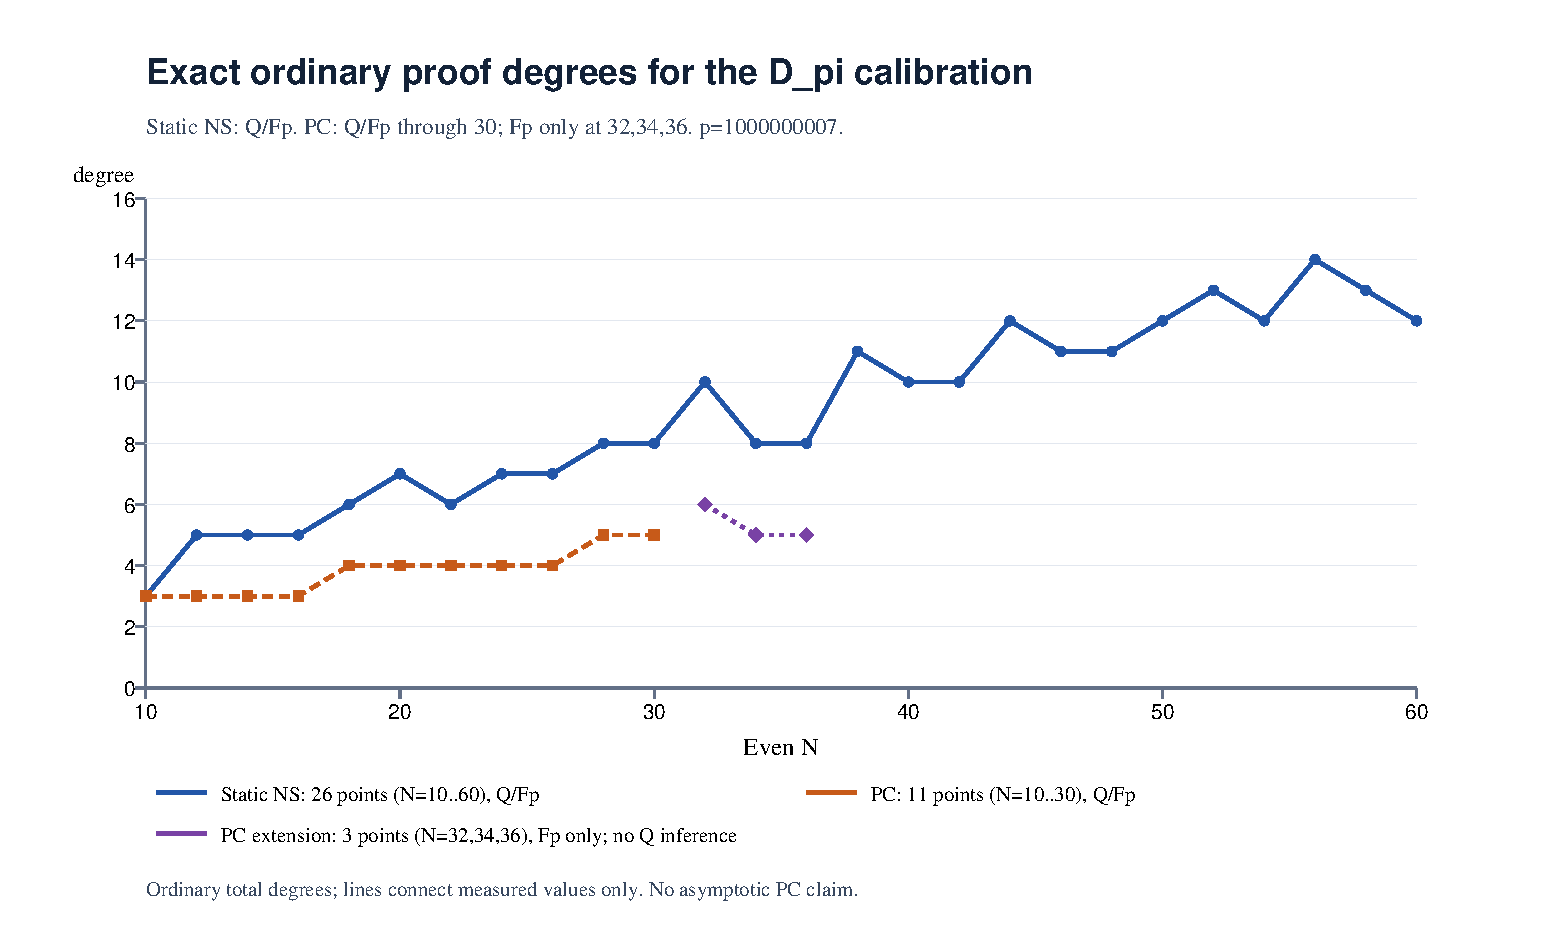
\includegraphics[width=.88\linewidth]{figures/degree_curve.pdf}
\caption{Existing finite degree plot. Static NS equality is measured over
$\mathbb Q$ and $\mathbb F_{1000000007}$ at even $N=10,\ldots,60$.
PC degrees agree over both fields at even $N=10,\ldots,30$; the points
$N=32,34,36$ are finite-field-only. The plot is evidence at these inputs,
not a universal upper bound or a rational transfer.\ev{ALG-DEGREE-FIGURE}}
\label{fig:degree}
\end{figure}

Grouping the existing CSV rows using $\alpha$ from the saved lower-bound
JSON finds the same PC degree whenever $\alpha$ repeats in these $14$
finite-field points. The complete observed groups are:
\begin{center}
\begin{tabular}{@{}lll@{}}
\toprule
$\alpha$ & $N$ & Observed PC degree\\
\midrule
$2$ & $10$ & $3$ \\
$4$ & $12,14,16$ & $3$ \\
$5$ & $18,22$ & $4$ \\
$6$ & $20,24,26$ & $4$ \\
$7$ & $28,30,34,36$ & $5$ \\
$9$ & $32$ & $6$ \\
\bottomrule
\end{tabular}
\end{center}
This is finite group consistency, not a universal dependence theorem or a
closed PC degree formula.\ev{ALG-PC-ALPHA-GROUPING}

The compiled ordinary-Q restriction sends a supplied $D_\pi$ PC refutation
to a genuine Boolean-knapsack refutation on $\alpha$ variables without
increasing ordinary line degree. The explicit external predicate
\texttt{KnapsackLowerBound} remains a hypothesis of its lower corollary.
That conditional corollary is out of scope and is recorded in Appendix B;
the partial lattice, coefficient and count-action lemmas do not remove
the hypothesis.\ev{ALG-PC-HYPOTHESIS}


\section{Obstruction catalogue}
Table~\ref{tab:obstructions} collects the specific failed implications and
restricted impossibility statements. Each row refers to the object defined
in the corresponding section. A common zero for one family rules out a
certificate for that family; it says nothing universal about all possible
families. A failed sign argument leaves other analytic arguments open.

\begin{table}[ht]\centering\footnotesize
\caption{Scope of the recorded obstructions.}\label{tab:obstructions}
\begin{tabular}{p{3.1cm}p{3.5cm}p{2.1cm}p{5.7cm}}
\toprule
Obstruction & Scope & Status & What it does not show\\
\midrule
Exact projection lacks a signed lower bound & True additive coefficient &
Compiled identities; open estimate & It does not supply a positive
prime-pair margin.\ev{R-ANALYTIC-GAP}\\
Absolute error control lacks cancellation & Quantization or truncation
envelopes & Mixed compiled/\allowbreak SOURCE & A small approximation radius does not
control the sign of the reference-minus-coefficient term.\ev{R-ANALYTIC-GAP}\\
Boundary term retained & Individual Mellin kernel & Compiled Lean &
Periodicity of the full trace does not delete each kernel boundary.\ev{R-BOUNDARY}\\
Positive definite reconstruction lacks paired mass & The recorded
restricted positive series & PAPER & Positivity alone does not imply a
uniform strictly positive additive coefficient.\ev{R-FEJER}\\
Negative direction of the reviewed kernel & Specific operator restriction
& PAPER & It does not exclude every operator method.\ev{R-KERNEL}\\
Cost of the proposed tail envelope & Particular written Mellin error
envelope & PAPER / SOURCE & It is not a lower bound for the true error or
for every evaluation algorithm.\ev{A-OBSTRUCTION-COST}\\
Finite arithmetic counterexamples and losses & The guarded block, mask,
completion, rank and Type-II groups in Appendix A & Compiled Lean &
They refute the specified intermediate claims, not the full analytic
programme.\ev{A-ARITHMETIC-OBSTRUCTIONS}\\
Circular or direct-pinning constraints & Calibration and named family
equations & Compiled/\allowbreak SOURCE guard & They do not provide new information
about the prime vector.\ev{R-ALGEBRAIC}\\
Common zeros & Specified Bertrand, divisor and literal families & Compiled
Lean / EVIDENCE & They do not exclude the complete certificate
route.\ev{R-ALGEBRAIC}\\
Growing certificate degree & Rational static full-count calibration &
Compiled lower bound & It does not forbid unbounded degree or a different
constraint family.\ev{R-DEGREE}\\
Finite computation has finite scope & One completed integer/CRT input &
EVIDENCE & It is not an all-input native refinement or an analytic
threshold theorem.\ev{R-NUMERICAL}\\
\bottomrule
\end{tabular}
\end{table}

The sieve parity limitation is classical background, not a new theorem of
this project.\cite{selberg1949}
The algebraic and analytic obstructions in this table have different
mechanisms; no implication between them is asserted merely because each
prevents a particular attempted argument.

\section{The finite computation at $N=10^8$}
\label{sec:numerical}

The saved numerical verdict concerns one input,
$N=100000000$, with transform length $K=134217728=2^{27}$ and
scale $S=288230376151711744=2^{58}$. It records
\status{EXACT\_NUMERICAL\_ARITHMETIC\_VALIDATED} for the equality of the
five-modulus CRT reconstruction, the direct canonical A32 integer sum and
the auxiliary B40 integer sum. The documentary numerical check is separate
from the compiled finite-field identities in Section~\ref{sec:analytic}.
It is not a fresh execution of the transform or the prime catalogue.
\ev{A-NUMERICAL}

\begin{center}
\begin{tabular}{rr}
\toprule Modulus & Saved residue\\\midrule
2013265921 & 577099750\\
2281701377 & 626366149\\
3221225473 & 232952773\\
3489660929 & 2618309304\\
3892314113 & 2671748987\\
\bottomrule
\end{tabular}
\end{center}

The stored CRT product and reconstructed integer are, respectively,
\begin{align*}
 P_{\mathrm{CRT}}&=200988950952742247103310192629436327377560928257,\\
 I_{10^8}&=14616354094337692277256326339388864358034646.
\end{align*}
The same integer is recorded for the direct A32 and B40 sums, with
actual difference zero. The saved catalogue contains 5761455 prime
records. The coefficient denominator is
\[
 S^2=83076749736557242056487941267521536.
\]
This denominator scales the quantized integer coefficient; the integer
itself is not the real von Mangoldt coefficient.\ev{A-NUMERICAL}

The saved logarithm-envelope numerators, over this denominator, are
\begin{align*}
 E_{\log}:&\quad1844674425817699235409551617,\\
 2E_{\log}:&\quad3689348851635398470819103234.
\end{align*}
Their recorded decimal values are approximately
\begin{align*}
 E_{\log}&\approx2.2204460714547736\cdot10^{-8},\\
 2E_{\log}&\approx4.4408921429095471\cdot10^{-8}.
\end{align*}
The joint radius is below $10^{-6}$. The real-coefficient enclosure theorem in
\nolinkurl{QuantizedLambdaEnvelope22} applies to its mathematical
canonical integer constructor. Connecting every native output to that
constructor would require the native-program refinement that the verdict
explicitly leaves unproved.\ev{A-NUMERICAL}\ev{A-LOG}

The verdict also explicitly leaves B40 real-logarithm refinement and the
Mellin coefficient-truncation chain unproved. It establishes neither the
required signed $D_N$ estimate nor a Goldbach conclusion. In particular,
this single coefficient computation is not a verification of every even
integer up to $10^8$, and equality of two saved integer sums does not make
either unproved analytic refinement automatic.\ev{A-NUMERICAL}


\section{What a sufficient approach would still require}
In the preserved analytic notation, $C_N$ is the von Mangoldt convolution
and includes proper prime powers, while $R_{\mathrm{ref}}$ is the reference
quantity of the existing balance framework. A signed estimate for
$R_{\mathrm{ref}}-C_N$ remains necessary within that framework, together
with the prime-power correction, boundary terms and its stated bridge
conditions. A coefficient representation or enclosure does not supply
that estimate.\ev{R-ANALYTIC-GAP}
An ingredient sensitive to the prime versus almost-prime distinction is
still required; invoking parity terminology alone provides no such input.

The analytic onset in the V3.1 framework is $\log N\ge10^{24}$.
The single finite computation at $N=10^8$ is outside this regime. The
published verification through $4\cdot10^{18}$ leaves the interval to that
analytic onset uncovered by the present corpus. No theorem or computation
in this report fills that interval.\ev{R-THRESHOLD}\cite{osilva2014}

For the algebraic route, a family would need genuinely sufficient
prime-valid information without circularly assuming the desired
nonvanishing, and an actual uniform identity with its ordinary degree
accounted for. Lower bounds for a calibration do not substitute for that
construction. The open matching static construction and the assumed
polynomial-calculus lower-bound predicate remain separate obligations.
\ev{R-DEGREE}\ev{R-PC}

\section{Reproducibility and archival scope}
The publication repository is
\url{https://github.com/seisner1967-hash/goldbach-horizon}.
The pre-publication repository snapshot is \texttt{f7e1fda19a97}; the
accepted algebraic proof snapshot is \texttt{e5c4e119473e}.
Their recorded toolchain is Lean~4.15.0 with Mathlib revision
\texttt{9837ca9d65d9}.\ev{R-REPRO}
At the appropriate pinned source snapshot the project build command is
\begin{center}\texttt{lake build}\end{center}
This manuscript preparation did not execute it. A successful auxiliary
build does not prove the unfinished frozen target.\ev{R-FROZEN}

The generated inventory records theorem names, the available axiom lists,
credit levels, source hashes and existing commit identifiers. Its scripts
derive tables from existing artifacts only. The algebraic
\texttt{AXIOMS.md} source and analytic audit records are identified in
\texttt{evidence\_map.json}. Appendix~\ref{app:inventory} explains their
coverage and records omissions rather than inventing missing credit.
\ev{R-REPRO}

The arXiv source bundle contains portable TeX, the compiled bibliography
and figures. Larger binary evidence is not included in this paper commit;
its hashes and scope are recorded for a separate author-managed release.
The source bundle does not need a local workspace path to compile.

\clearpage
\appendix
\section{Generated Lean inventory}\label{app:inventory}
The tables and companion CSV/JSON inventories are generated from existing
source declarations and audit artifacts. Definitions are identified as
definitions; auxiliary declaration counts are not theorem counts. A
declaration listed with SOURCE status is not listed as an established
theorem. Explicit local hypotheses are retained in the informal statement.
The table column ``axioms'' records what the available audit actually
prints; an absent per-declaration audit is not filled by inference.
\subsection{Analytic inventory from existing Judge artifacts}
\label{app:analytic-inventory}
The electronic files \texttt{analytic\_inventory.json} and \texttt{analytic\_lean\_inventory.csv} list every extracted axiom-audit row, its declaration kind, recorded axioms, textual declaration header, source and receipt paths, full hashes and existing repository commit. The header is extracted Lean text, not an elaborated type; surrounding section variables and hypotheses remain in the pinned source. A missing separate paraphrase is explicitly labelled. These tables are generated by \texttt{generate\_analytic\_inventory.py} from existing artifacts only.
The recorded official counter is 88 modules and 1,488 mixed historical entries. The exhaustive axiom-row extraction gives 1,768 rows: 1,222 historical and 546 from round 22. The historical counter counts 942 theorems, while later axiom rows also contain definitions and structures. Consequently neither 1,488 nor 1,768 is presented as a theorem count. Definitions without an individual axiom row are not assigned an invented empty axiom list.
The tables below select one recorded theorem per module and give a human paraphrase of its scope. They do not replace the original hypotheses in the pinned source. The electronic inventory retains all 1,768 rows. Commit \texttt{f7e1fda19a97} contains the existing public artifacts; source and receipt hashes identify their exact bytes. The axiom abbreviations are P=\texttt{propext}, C=\texttt{Classical.choice}, Q=\texttt{Quot.sound}. A partial label means module-row PASS in a globally FAILED batch. Batches 6, 7, 8, 9, 11 and 26 have such retained rows; failed or uninvoked rows are excluded.\ev{A-INVENTORY-COUNTS}\ev{A-PARTIAL-BATCHES}
\begin{center}\scriptsize
\begin{tabular}{@{}p{0.20\textwidth}p{0.52\textwidth}p{0.19\textwidth}@{}}
\toprule Module & Selected theorem and informal statement & Axioms; credit; commit; source SHA\\\midrule
Parity\allowbreak{}Weights & \nolinkurl{concrete_prime_triprime_same_parity}. The prime 101 and the composite 101*103*107 have the same odd parity weight; the composite lies between 100 and 100000000 and has no prime divisor at most 100. & P,C,Q; Compiled Lean; \texttt{f7e1fda}; \texttt{8c4954596ac6}\\
Quartic\allowbreak{}Mobius & \nolinkurl{weighted_boundary_identity_real}. For arguments between alpha and N with N at most alpha\textasciicircum{}4, the weighted Mobius sum equals the stated combination of short double, cubic and quartic divisor sums. & P,C,Q; Compiled Lean; \texttt{f7e1fda}; \texttt{1c370324b3d9}\\
Chen\allowbreak{}Weight & \nolinkurl{weighted_prime_identity_real}. Under the quartic cap and the absence of prime factors at most alpha, the finite weighted Chen expression equals the corresponding prime-indicator sum. & P,C,Q; Compiled Lean; \texttt{f7e1fda}; \texttt{65a38665aeae}\\
Multifibre\allowbreak{}Obstruction & \nolinkurl{literalFourSiteBlock_neg}. The explicitly defined four-site block is negative. & P,C,Q; Compiled Lean; \texttt{f7e1fda}; \texttt{93a5d98934c2}\\
\bottomrule\end{tabular}\end{center}
\begin{center}\scriptsize
\begin{tabular}{@{}p{0.20\textwidth}p{0.52\textwidth}p{0.19\textwidth}@{}}
\toprule Module & Selected theorem and informal statement & Axioms; credit; commit; source SHA\\\midrule
Quotient\allowbreak{}Gauss & \nolinkurl{weighted_transform_real_part}. Under the finite-ring character assumptions in the source, the weighted real part of the quotient Kloosterman transform equals the squared Gauss-sum expression. & P,C,Q; Compiled Lean; \texttt{f7e1fda}; \texttt{a8628dc031cf}\\
Affine\allowbreak{}HHObstruction & \nolinkurl{concrete_mixed_level_displacement}. The displayed mixed difference of four concrete rational hhLevel values equals 1040. & P,C,Q; Compiled Lean; \texttt{f7e1fda}; \texttt{9e3274b7f220}\\
Composite\allowbreak{}Completion & \nolinkurl{zero_frequency_is_nonunit}. In a nontrivial ZMod ring, zero belongs to the set of nonunits. & P,C,Q; Compiled Lean; \texttt{f7e1fda}; \texttt{af643e3021ee}\\
Determinant\allowbreak{}Coordinates & \nolinkurl{concrete_expanded_tuple_sign_change}. The two displayed expanded determinant tuples have signs +1 and -1 respectively. & P,C,Q; Compiled Lean; \texttt{f7e1fda}; \texttt{aafce8f549d2}\\
\bottomrule\end{tabular}\end{center}
\begin{center}\scriptsize
\begin{tabular}{@{}p{0.20\textwidth}p{0.52\textwidth}p{0.19\textwidth}@{}}
\toprule Module & Selected theorem and informal statement & Axioms; credit; commit; source SHA\\\midrule
Unit\allowbreak{}Supported\allowbreak{}Completion & \nolinkurl{double_unit_supported_completion}. For two functions vanishing on nonunits, the product of their unit-frequency moments satisfies the stated Gauss-normalized completion identity. & P,C,Q; Compiled Lean; \texttt{f7e1fda}; \texttt{7d84fa747313}\\
Prime\allowbreak{}Cofactor\allowbreak{}Identity & \nolinkurl{source_prime_bracket_cofactor}. For an admissible prime/cofactor representation with the original quotient cap and unit condition, the source prime bracket has the explicit Mobius-logarithm factorization. & P,C,Q; Compiled Lean; \texttt{f7e1fda}; \texttt{a31895518a60}\\
Short\allowbreak{}Divisor\allowbreak{}Complement & \nolinkurl{at_one}. At argument one, the capped divisor kernel satisfies the displayed complementary short-divisor identity, for arbitrary natural caps. & P,C,Q; Compiled Lean; \texttt{f7e1fda}; \texttt{25f38fcb6f84}\\
Squarefree\allowbreak{}Lcm\allowbreak{}Coefficient & \nolinkurl{squarefree_lcm_coefficient_unit}. For squarefree P coprime to N and r dividing P, the unit-masked lcm/totient sum equals the explicit finite Euler product divided by r. & P,C,Q; Compiled Lean; \texttt{f7e1fda}; \texttt{f791b4be0f73}\\
\bottomrule\end{tabular}\end{center}
\begin{center}\scriptsize
\begin{tabular}{@{}p{0.20\textwidth}p{0.52\textwidth}p{0.19\textwidth}@{}}
\toprule Module & Selected theorem and informal statement & Axioms; credit; commit; source SHA\\\midrule
Three\allowbreak{}Adic\allowbreak{}Prime\allowbreak{}Pairing & \nolinkurl{actual_principal_partition}. Under the recorded prime, ordering, coprimality and cap assumptions, the actual principal sum splits exactly into entropy, paired, singleton and geometric-face terms. & P,C,Q; Compiled Lean; \texttt{f7e1fda}; \texttt{b3c22b714566}\\
Prime\allowbreak{}Semiprime\allowbreak{}Switch & \nolinkurl{actual_admissible_switch}. For the specified admissible prime-to-semiprime switch, the two source brackets satisfy an exact logarithmic difference identity retaining both harmonic kernels. & P,C,Q; Compiled Lean; \texttt{f7e1fda}; \texttt{21462365bb2f}\\
Harmonic\allowbreak{}Kernel\allowbreak{}Variation & \nolinkurl{actual_kernel_abs_variation}. For positive front and arguments, ordered cofactors and prime complements beyond Q, harmonic-kernel variation is bounded by the two explicit finite logarithm/totient sums. & P,C,Q; Compiled Lean; \texttt{f7e1fda}; \texttt{7bc1ee92e0e9}\\
Least\allowbreak{}Missing\allowbreak{}Prime\allowbreak{}Margin & \nolinkurl{large_prime_margin}. For every natural p at least 13, the displayed harmonic-minus-logarithm expression is at least 1/144; primality is not required. & P,C,Q; Compiled Lean; \texttt{f7e1fda}; \texttt{e1dbd4f8a68b}\\
\bottomrule\end{tabular}\end{center}
\begin{center}\scriptsize
\begin{tabular}{@{}p{0.20\textwidth}p{0.52\textwidth}p{0.19\textwidth}@{}}
\toprule Module & Selected theorem and informal statement & Axioms; credit; commit; source SHA\\\midrule
Euler\allowbreak{}Anchor & \nolinkurl{canonical_least_missing_prime_margin}. For nonzero even N and the stated lower bound on the twin constant, the singular series exceeds the logarithm of the least missing odd prime by at least 1/144. & P,C,Q; Compiled Lean; \texttt{f7e1fda}; \texttt{88bbbb4d8e49}\\
Four\allowbreak{}Form\allowbreak{}Roots & \nolinkurl{zero_mem_actualRoots}. Zero is a root of the actual four-form product over ZMod, with the source parameters retained. & P,C,Q; Compiled Lean; \texttt{f7e1fda}; \texttt{49cbf93fd8eb}\\
Powerset\allowbreak{}Moment & \nolinkurl{weighted_moment}. For nonnegative finite subset weights, the first weighted powerset moment factors as a product times the sum of h/(1+h) contributions. & P,C,Q; Compiled Lean; \texttt{f7e1fda}; \texttt{971f351decef}\\
Selberg\allowbreak{}Four\allowbreak{}Forms & \nolinkurl{weight_zero_outside}. If every element of P is at least one, a divisor subset outside the defined Selberg support has zero weight. & P,C,Q; Compiled Lean; \texttt{f7e1fda}; \texttt{b1b658aa92f8}\\
\bottomrule\end{tabular}\end{center}
\begin{center}\scriptsize
\begin{tabular}{@{}p{0.20\textwidth}p{0.52\textwidth}p{0.19\textwidth}@{}}
\toprule Module & Selected theorem and informal statement & Axioms; credit; commit; source SHA\\\midrule
Four\allowbreak{}Form\allowbreak{}Truncation & \nolinkurl{primeSupport_mono}. The prime support at cutoff y is contained in that at cutoff z whenever y is at most z. & P,C,Q; Compiled Lean; \texttt{f7e1fda}; \texttt{577ff585207e}\\
Four\allowbreak{}Form\allowbreak{}Collision\allowbreak{}Loss & \nolinkurl{primeBase_positive}. The defined collision base is strictly positive at every prime. & P,C,Q; Compiled Lean; \texttt{f7e1fda}; \texttt{000cade7cac3}\\
Separated\allowbreak{}Type\allowbreak{}II & \nolinkurl{xi_bound}. The defined finite coefficient xi has absolute value at most one for every finite E and natural v. & P,C,Q; Compiled Lean; \texttt{f7e1fda}; \texttt{4513f3323bbf}\\
Separated\allowbreak{}Type\allowbreak{}IIPrice & \nolinkurl{weighted_one_is_adversarial}. The separated bilinear sum with constant weight one equals the defined adversarial sum. & P,C,Q; Compiled Lean; \texttt{f7e1fda}; \texttt{dd971712c281}\\
\bottomrule\end{tabular}\end{center}
\begin{center}\scriptsize
\begin{tabular}{@{}p{0.20\textwidth}p{0.52\textwidth}p{0.19\textwidth}@{}}
\toprule Module & Selected theorem and informal statement & Axioms; credit; commit; source SHA\\\midrule
Separated\allowbreak{}Type\allowbreak{}IICount & \nolinkurl{units_inclusion}. For nonzero H, the count of elements coprime to H equals its Mobius divisor inclusion-exclusion sum. & P,C,Q; Compiled Lean; \texttt{f7e1fda}; \texttt{55ac598030d5}\\
Separated\allowbreak{}Type\allowbreak{}IILower & \nolinkurl{omitted_ratio_lower_R5}. Under the explicit conductor, interval, unit-count and three front/density guards, the omitted-to-unit ratio is at least density(H*ell)/(16*ell). & P,C,Q; Compiled Lean; \texttt{f7e1fda}; \texttt{5676b1d3be3a}\\
Double\allowbreak{}Extraction\allowbreak{}Arithmetic & \nolinkurl{witnesses_distinct}. The two constructed witnesses of an admissible Cell are distinct. & P,C,Q; Compiled Lean; \texttt{f7e1fda}; \texttt{be85b2d59e5a}\\
Divided\allowbreak{}Four\allowbreak{}Forms & \nolinkurl{slopeProduct_eq}. The product of the divided-form slopes equals minus e times the anchor times the cube of the modulus. & P,C,Q; Compiled Lean; \texttt{f7e1fda}; \texttt{613dba073eb1}\\
\bottomrule\end{tabular}\end{center}
\begin{center}\scriptsize
\begin{tabular}{@{}p{0.20\textwidth}p{0.52\textwidth}p{0.19\textwidth}@{}}
\toprule Module & Selected theorem and informal statement & Axioms; credit; commit; source SHA\\\midrule
Divided\allowbreak{}Root\allowbreak{}Counts & \nolinkurl{witness1_q_cast_ne_zero}. For an admissible Cell, q is nonzero modulo the second constructed witness. & P,C,Q; Compiled Lean; \texttt{f7e1fda}; \texttt{f7c4a4e4f2ca}\\
Divided\allowbreak{}Selberg\allowbreak{}Bridge & \nolinkurl{switch_weighted_moment}. For an admissible Cell and nonsaturated local root counts, the switched powerset logarithmic moment equals its Euler product times the local-density sum. & P,C,Q; Compiled Lean; \texttt{f7e1fda}; \texttt{2b5f1edaaab6}\\
Rank\allowbreak{}Calibration\allowbreak{}Face & \nolinkurl{three_small_primes_face_excludes_physicalMask}. Three distinct prime divisors whose squares are at most the front exclude the defined arithmetic mask when their product divides the conductor-weighted argument. & P,C,Q; Compiled Lean; \texttt{f7e1fda}; \texttt{8bd774d17ae5}\\
Rank\allowbreak{}Calibration\allowbreak{}Price & \nolinkurl{weighted_rank_price_decomposition}. The finite aggregate rank quantity decomposes exactly through an intermediate set into the remaining quantity and two price terms. & P,C,Q; Compiled Lean; \texttt{f7e1fda}; \texttt{ce00b2b3d416}\\
\bottomrule\end{tabular}\end{center}
\begin{center}\scriptsize
\begin{tabular}{@{}p{0.20\textwidth}p{0.52\textwidth}p{0.19\textwidth}@{}}
\toprule Module & Selected theorem and informal statement & Axioms; credit; commit; source SHA\\\midrule
Rank\allowbreak{}Calibration\allowbreak{}Arithmetic & \nolinkurl{squarefree_subdivisor_reconstruction}. If d and d' are squarefree, k divides d and k' divides d', equality d*k=d'*k' forces equality of both pairs. & P,C,Q; Compiled Lean; \texttt{f7e1fda}; \texttt{3ac4ec121db2}\\
Rank\allowbreak{}Calibration\allowbreak{}Unit\allowbreak{}Loss & \nolinkurl{small_prime_dvd_small_conductor}. Either designated prime c or r divides the defined small conductor whenever it is at most the cutoff R. & P,C,Q; Compiled Lean; \texttt{f7e1fda}; \texttt{2a3eaafd2e74}\\
Rank\allowbreak{}Calibration\allowbreak{}Euler & \nolinkurl{weighted_unit_inclusion}. For nonzero K, a finite sum over units modulo K equals its Mobius-weighted divisor inclusion-exclusion sum. & P,C,Q; Compiled Lean; \texttt{f7e1fda}; \texttt{30449aa225e9}\\
Rank\allowbreak{}Calibration\allowbreak{}Estimator & \nolinkurl{normalized_density_error_bound}. For A at most J and positive ideal denominator, the difference of normalized A/J and A/ideal is bounded by the denominator discrepancy divided by ideal. & P,C,Q; Compiled Lean; \texttt{f7e1fda}; \texttt{2d175fb99479}\\
\bottomrule\end{tabular}\end{center}
\begin{center}\scriptsize
\begin{tabular}{@{}p{0.20\textwidth}p{0.52\textwidth}p{0.19\textwidth}@{}}
\toprule Module & Selected theorem and informal statement & Axioms; credit; commit; source SHA\\\midrule
Terminal\allowbreak{}Prime\allowbreak{}Extraction & \nolinkurl{terminal_factorization}. For n at least two, the constructed cofactor multiplied by the terminal prime equals n. & P,C,Q; Compiled Lean; \texttt{f7e1fda}; \texttt{e7e6e458143b}\\
Balanced\allowbreak{}Resource\allowbreak{}Switch & \nolinkurl{three_strata}. Every factor tuple falls into one of the three stated conductor ranges, separated by B and the square comparison with N. & P,C,Q; Compiled Lean; \texttt{f7e1fda}; \texttt{310338aef835}\\
Signed\allowbreak{}Hyperbolic\allowbreak{}CRT & \nolinkurl{unpack_encode}. For an admissible resource cell, unpacking the signed encoding recovers the original encoding. & P,C,Q; Compiled Lean; \texttt{f7e1fda}; \texttt{69d0e23f36b1}\\
Non\allowbreak{}SSBracket\allowbreak{}Switch & \nolinkurl{theta_coordinate_reindex}. The finite theta-bracket sum on the defined admissible domain equals its factor-coordinate reindexing. & P,C,Q; Compiled Lean; \texttt{f7e1fda}; \texttt{8d4cc04aa370}\\
\bottomrule\end{tabular}\end{center}
\begin{center}\scriptsize
\begin{tabular}{@{}p{0.20\textwidth}p{0.52\textwidth}p{0.19\textwidth}@{}}
\toprule Module & Selected theorem and informal statement & Axioms; credit; commit; source SHA\\\midrule
Rank\allowbreak{}Two\allowbreak{}Harmonic & \nolinkurl{unordered_pair_moment}. The ordered half of a symmetric weighted pair sum equals one half of the sum of the squared total and the diagonal square sum. & P,C,Q; Compiled Lean; \texttt{f7e1fda}; \texttt{06cbe631518b}\\
Odd\allowbreak{}Bonferroni\allowbreak{}Arithmetic & \nolinkurl{truncated_choose_zero}. For every truncation order, the alternating binomial sum at zero equals one. & P,C,Q; Compiled Lean; \texttt{f7e1fda}; \texttt{e5348cf2301c}\\
Least\allowbreak{}Factor\allowbreak{}Composite & \nolinkurl{square_quotient}. For prime p, the least-prime quotient of p squared equals p. & P,C,Q; Compiled Lean; \texttt{f7e1fda}; \texttt{4c114ae1b730}\\
Switched\allowbreak{}Selberg\allowbreak{}Weight & \nolinkurl{totientDensity_properties}. For even N, the totient density at every prime in the switched support is strictly between zero and one. & P,C,Q; Compiled Lean; \texttt{f7e1fda}; \texttt{c0a640773636}\\
\bottomrule\end{tabular}\end{center}
\begin{center}\scriptsize
\begin{tabular}{@{}p{0.20\textwidth}p{0.52\textwidth}p{0.19\textwidth}@{}}
\toprule Module & Selected theorem and informal statement & Axioms; credit; commit; source SHA\\\midrule
Physical\allowbreak{}Composite\allowbreak{}Subtraction & \nolinkurl{physicalRaw_theta_difference}. The defined raw arithmetic mass equals its prime mass plus the proper-prime-power difference. & P,C,Q; Compiled Lean; \texttt{f7e1fda}; \texttt{3d6ef57fd5fc}\\
Composite\allowbreak{}APConductor & \nolinkurl{totient_product_kernel}. For a finite set of primes, the Selberg product of totient densities equals the reciprocal totient of the prime product. & P,C,Q; Compiled Lean; \texttt{f7e1fda}; \texttt{04809ca5369c}\\
Switched\allowbreak{}Incidence\allowbreak{}Estimator & \nolinkurl{switchedIncidence_reference_price}. For even N and positive cutoff, the prime incidence minus its reference is bounded by the constructed main terms, both absolute remainders and the retained large-composite subtraction. & P,C,Q; Compiled Lean; \texttt{f7e1fda}; \texttt{7ea6cc850698}\\
Friable\allowbreak{}Physical\allowbreak{}Prefix & \nolinkurl{smooth_large_has_actual_band_divisor}. A Y-smooth integer n at least D has a divisor in the defined divisor band when D>1 and Y>0. & P,C,Q; Compiled Lean; \texttt{f7e1fda}; \texttt{4286a04e155a}\\
\bottomrule\end{tabular}\end{center}
\begin{center}\scriptsize
\begin{tabular}{@{}p{0.20\textwidth}p{0.52\textwidth}p{0.19\textwidth}@{}}
\toprule Module & Selected theorem and informal statement & Axioms; credit; commit; source SHA\\\midrule
Friable\allowbreak{}Euler\allowbreak{}Rankin & \nolinkurl{tau_prime_pow}. At a prime power p\textasciicircum{}k, the divisor-counting function tau equals k+1. & P,C,Q; Compiled Lean; \texttt{f7e1fda}; \texttt{df9ddafb7b49}\\
Friable\allowbreak{}Kernel\allowbreak{}Envelope & \nolinkurl{totientInverseSum_mono}. The finite reciprocal-totient sum is monotone in its natural cutoff. & P,C,Q; Compiled Lean; \texttt{f7e1fda}; \texttt{80051a67fa9d}\\
Friable\allowbreak{}Prime\allowbreak{}Harmonic & \nolinkurl{pseries_tsum_le_one_add_inv}. For positive sigma, the nonnegative p-series with exponent 1+sigma is at most 1+1/sigma. & P,C,Q; Compiled Lean; \texttt{f7e1fda}; \texttt{53df26ec4a58}\\
Friable\allowbreak{}Totient\allowbreak{}Envelope & \nolinkurl{weightedInverseTotient_multiplicative}. The defined weighted inverse-totient arithmetic function is multiplicative. & P,C,Q; Compiled Lean; \texttt{f7e1fda}; \texttt{14419032ada2}\\
\bottomrule\end{tabular}\end{center}
\begin{center}\scriptsize
\begin{tabular}{@{}p{0.20\textwidth}p{0.52\textwidth}p{0.19\textwidth}@{}}
\toprule Module & Selected theorem and informal statement & Axioms; credit; commit; source SHA\\\midrule
Friable\allowbreak{}Physical\allowbreak{}Payment & \nolinkurl{uniqueResources1_subset_smoothInterval}. The second set of unique smooth resources is contained in the defined smooth interval. & P,C,Q; Compiled Lean; \texttt{f7e1fda}; \texttt{b4b108b42406}\\
Friable\allowbreak{}Physical\allowbreak{}Demand & \nolinkurl{actual_theta_demand_abs_le_seven_log_cube}. Under the recorded structural support and front guards with log N at least one, the theta bracket has absolute value at most 7(log N)\textasciicircum{}3. & P,C,Q; Compiled Lean; \texttt{f7e1fda}; \texttt{b02cb0aced0d}\\
Friable\allowbreak{}Demand\allowbreak{}Aggregation & \nolinkurl{friableRank_support}. Membership in the defined friable rank implies structural support and smoothness of at least one of its two resources. & P,C,Q; Compiled Lean; \texttt{f7e1fda}; \texttt{b564591ccb21}\\
Friable\allowbreak{}Source\allowbreak{}Geometry & \nolinkurl{source_u_pos}. Under the defined source-onset condition, sourceU is positive. & P,C,Q; Compiled Lean; \texttt{f7e1fda}; \texttt{bc249b736e46}\\
\bottomrule\end{tabular}\end{center}
\begin{center}\scriptsize
\begin{tabular}{@{}p{0.20\textwidth}p{0.52\textwidth}p{0.19\textwidth}@{}}
\toprule Module & Selected theorem and informal statement & Axioms; credit; commit; source SHA\\\midrule
Friable\allowbreak{}Source\allowbreak{}Budget & \nolinkurl{source_rank_front_le_two_N}. Under the source-onset condition, the product of the defined three source fronts is at most 2N. & P,C,Q; Compiled Lean; \texttt{f7e1fda}; \texttt{9dd811fe823f}\\
Epstein\allowbreak{}Kernel22 & \nolinkurl{boundary_deficit_bounds}. For positive a and u, the defined boundary deficit lies between zero and a\textasciicircum{}2/(2u\textasciicircum{}2). & P,C,Q; Compiled Lean; \texttt{f7e1fda}; \texttt{b465bf53b124}\\
Epstein\allowbreak{}Finite22 & \nolinkurl{finiteShiftIntegral_formula}. For positive y and nonzero integer m, the finite shifted integral equals the stated weight-scaled endpoint sum. & P,C,Q; Compiled Lean; \texttt{f7e1fda}; \texttt{fb6205d1d88b}\\
Epstein\allowbreak{}Unfold22 & \nolinkurl{unfoldFullRealThreeHalves_natAbs}. For positive y and nonzero integer m, the infinite shifted integral equals 2/(|m|\textasciicircum{}2 sqrt(y)). & P,C,Q; Compiled Lean; \texttt{f7e1fda}; \texttt{79384d3502ab}\\
\bottomrule\end{tabular}\end{center}
\begin{center}\scriptsize
\begin{tabular}{@{}p{0.20\textwidth}p{0.52\textwidth}p{0.19\textwidth}@{}}
\toprule Module & Selected theorem and informal statement & Axioms; credit; commit; source SHA\\\midrule
Epstein\allowbreak{}Tail22 & \nolinkurl{continuousOn_truncationEnvelopeReal}. The defined real truncation envelope is continuous on the parameter domain where its second coordinate exceeds the fixed cutoff q. & P,C,Q; Compiled Lean; \texttt{f7e1fda}; \texttt{5f9d3f180df2}\\
Gamma\allowbreak{}Prerequisites22 & \nolinkurl{Gamma_strip_exponential_bound}. The actual Gamma function has norm at most 2 exp(-pi|Im s|/4) throughout the closed strip 1<=Re s<=2. & P,C,Q; Compiled Lean; \texttt{f7e1fda}; \texttt{9f5e5fe14d18}\\
Gamma\allowbreak{}Derivative22 & \nolinkurl{Gamma_derivative_strip_exponential_bound}. The actual derivative of Gamma has norm at most 19 exp(-pi|Im s|/4) throughout the same closed strip. & P,C,Q; Compiled Lean; \texttt{f7e1fda}; \texttt{026ced6097c7}\\
Gamma\allowbreak{}Psi\allowbreak{}Core22 & \nolinkurl{betaDifference_eq_integral}. For Re z>0 and real w>0, the beta-integral difference equals the integral of the defined difference integrand on (0,1). & P,C,Q; Compiled Lean; \texttt{f7e1fda}; \texttt{450962be9526}\\
\bottomrule\end{tabular}\end{center}
\begin{center}\scriptsize
\begin{tabular}{@{}p{0.20\textwidth}p{0.52\textwidth}p{0.19\textwidth}@{}}
\toprule Module & Selected theorem and informal statement & Axioms; credit; commit; source SHA\\\midrule
Gamma\allowbreak{}Psi\allowbreak{}Beta\allowbreak{}Limit22 & \nolinkurl{gammaPsi_eq_beta_integral}. For Re z>0, the actual logarithmic derivative of Gamma equals minus Euler's constant plus its beta-integrand integral on (0,1). & P,C,Q; Compiled Lean; \texttt{f7e1fda}; \texttt{b4adf3ac71dd}\\
Gamma\allowbreak{}Psi\allowbreak{}Integral22 & \nolinkurl{gammaPsi_eq_exp_integral}. For Re z>0, the logarithmic derivative of Gamma equals minus Euler's constant plus the defined exponential integral over positive reals. & P,C,Q; Compiled Lean; \texttt{f7e1fda}; \texttt{3f254cdfeee3}\\
Gamma\allowbreak{}Box\allowbreak{}Bounds22 & \nolinkurl{gammaBoxRadius_continuousAt}. The defined four-parameter Gamma-box radius is jointly continuous at every point whose Y coordinate is positive. & P,C,Q; Compiled Lean; \texttt{f7e1fda}; \texttt{4874192b1c2c}\\
Gamma\allowbreak{}Contour\allowbreak{}Component22 & \nolinkurl{gammaContourEnvelope_continuous}. The defined two-parameter Gamma contour envelope is continuous. & P,C,Q; Compiled Lean; \texttt{f7e1fda}; \texttt{891454d4714e}\\
\bottomrule\end{tabular}\end{center}
\begin{center}\scriptsize
\begin{tabular}{@{}p{0.20\textwidth}p{0.52\textwidth}p{0.19\textwidth}@{}}
\toprule Module & Selected theorem and informal statement & Axioms; credit; commit; source SHA\\\midrule
Zeta\allowbreak{}Euler\allowbreak{}Direct22 & \nolinkurl{contourZeta_ne_zero_on_right}. The actual Riemann zeta function is nonzero for Re s>1. & P,C,Q; partial row PASS; \texttt{f7e1fda}; \texttt{0d790ed67706}\\
Zeta\allowbreak{}Reflection22 & \nolinkurl{contourZeta_logDeriv_reflection}. On -1<Re s<0, the zeta logarithmic derivative equals the contour-chi logarithmic derivative minus the reflected zeta logarithmic derivative. & P,C,Q; partial row PASS; \texttt{f7e1fda}; \texttt{cc39bd76e008}\\
Gamma\allowbreak{}Psi\allowbreak{}Duplication22 & \nolinkurl{gammaPsi_duplication}. For Re z>0, the Gamma logarithmic derivative satisfies psi(z)+psi(z+1/2)=2psi(2z)-2log 2. & P,C,Q; partial row PASS; \texttt{f7e1fda}; \texttt{0491177c6cfc}\\
Gamma\allowbreak{}Psi\allowbreak{}Reflection22 & \nolinkurl{gammaPsi_shift_reflection}. On -1<Re s<0, the indicated shifted Gamma-logarithmic-derivative difference equals 1/s minus the cotangent term. & P,C,Q; partial row PASS; \texttt{f7e1fda}; \texttt{a931bbceb530}\\
\bottomrule\end{tabular}\end{center}
\begin{center}\scriptsize
\begin{tabular}{@{}p{0.20\textwidth}p{0.52\textwidth}p{0.19\textwidth}@{}}
\toprule Module & Selected theorem and informal statement & Axioms; credit; commit; source SHA\\\midrule
Contour\allowbreak{}Chi\allowbreak{}Psi22 & \nolinkurl{contourChi_logDeriv_eq_pair_integral}. On -1<Re s<0, the contour-chi logarithmic derivative equals log pi plus Euler's constant, 1/s and the actual paired integral. & P,C,Q; partial row PASS; \texttt{f7e1fda}; \texttt{30c44bb1e376}\\
Thermal\allowbreak{}Projection\allowbreak{}Envelope22 & \nolinkurl{thermalContinuousProjection_error_le}. For a>0 and natural N,M, the full-versus-partial circle projection error is bounded by the constructed projectionErrorEnvelope. & P,C,Q; partial row PASS; \texttt{f7e1fda}; \texttt{77cdab8bed77}\\
Thermal\allowbreak{}Projection\allowbreak{}Identity22 & \nolinkurl{thermalContinuousProjection_eq_vonMangoldt_sum}. For a>0 and natural N, the continuous circle projection equals the genuine von Mangoldt additive coefficient, including prime powers. & P,C,Q; Compiled Lean; \texttt{f7e1fda}; \texttt{8bb1eb5ec6ab}\\
Discrete\allowbreak{}Thermal\allowbreak{}Projection22 & \nolinkurl{sampled_trueCircle_eq_coefficient}. For N<=M and K>max(N,2M-N), the finite sampled projector equals the genuine coefficient for every real damping parameter a. & P,C,Q; Compiled Lean; \texttt{f7e1fda}; \texttt{f24c702b0a6c}\\
\bottomrule\end{tabular}\end{center}
\begin{center}\scriptsize
\begin{tabular}{@{}p{0.20\textwidth}p{0.52\textwidth}p{0.19\textwidth}@{}}
\toprule Module & Selected theorem and informal statement & Axioms; credit; commit; source SHA\\\midrule
Rational\allowbreak{}Log\allowbreak{}Quantization22 & \nolinkurl{quantizedLog_precision}. For 2<=p<=100000000, the fixed rational log constructor has absolute error at most 1/gridScale. & P,C,Q; Compiled Lean; \texttt{f7e1fda}; \texttt{dfabcabf39ec}\\
Quantized\allowbreak{}Lambda\allowbreak{}Envelope22 & \nolinkurl{coefficient_error_bound}. For N<=100000000, the genuine coefficient differs from the scaled canonical integer coefficient by at most the explicit errorEnvelope. & P,C,Q; Compiled Lean; \texttt{f7e1fda}; \texttt{526354f4b960}\\
Finite\allowbreak{}Field\allowbreak{}Projection22 & \nolinkurl{fixed_A32_projection}. Over a prime field larger than 2\textasciicircum{}27, a root of order 2\textasciicircum{}27 gives the fixed canonical integer coefficient modulo that prime. & P,C,Q; Compiled Lean; \texttt{f7e1fda}; \texttt{2b1cc267ce78}\\
Thermal\allowbreak{}Gamma\allowbreak{}Mellin\allowbreak{}Inverse22 & \nolinkurl{real_exp_eq_Gamma_integral}. For real x>0, exp(-x) equals the normalized actual Gamma inversion integral on Re s=2. & P,C,Q; Compiled Lean; \texttt{f7e1fda}; \texttt{daad8b5d5fb1}\\
\bottomrule\end{tabular}\end{center}
\begin{center}\scriptsize
\begin{tabular}{@{}p{0.20\textwidth}p{0.52\textwidth}p{0.19\textwidth}@{}}
\toprule Module & Selected theorem and informal statement & Axioms; credit; commit; source SHA\\\midrule
Concrete\allowbreak{}NTTRoots22 & \nolinkurl{primitive_3892314113}. The specified bank root modulo the certified prime 3892314113 has exact multiplicative order 2\textasciicircum{}27. & P,C,Q; Compiled Lean; \texttt{f7e1fda}; \texttt{16c414a5d2f0}\\
Concrete\allowbreak{}NTTA32Projection22 & \nolinkurl{projection_3892314113}. The specified finite-field projector modulo 3892314113 returns the canonical integer coefficient at N=100000000. & P,C,Q; Compiled Lean; \texttt{f7e1fda}; \texttt{cefc07197945}\\
Angular\allowbreak{}Mellin\allowbreak{}Border22 & \nolinkurl{angularBorder_one_ne_zero}. For a>0 and natural N>0, the explicit angular boundary term at q=1 is nonzero. & P,C,Q; Compiled Lean; \texttt{f7e1fda}; \texttt{601a3360ff92}\\
Complex\allowbreak{}Gamma\allowbreak{}Mellin\allowbreak{}Local22 & \nolinkurl{complexGammaInverse_real}. The defined complex Gamma inverse agrees with exp(-x) on every positive real x. & P,C,Q; partial row PASS; \texttt{f7e1fda}; \texttt{e54cac5b2ab3}\\
\bottomrule\end{tabular}\end{center}
\begin{center}\scriptsize
\begin{tabular}{@{}p{0.20\textwidth}p{0.52\textwidth}p{0.19\textwidth}@{}}
\toprule Module & Selected theorem and informal statement & Axioms; credit; commit; source SHA\\\midrule
Complex\allowbreak{}Gamma\allowbreak{}Mellin\allowbreak{}Holomorphy22 & \nolinkurl{complex_exp_eq_Gamma_integral}. For Re w>0, exp(-w) equals the normalized actual Gamma integral with principal complex powers. & P,C,Q; Compiled Lean; \texttt{f7e1fda}; \texttt{b8b69c16cdbe}\\
Complex\allowbreak{}Gamma\allowbreak{}Mellin\allowbreak{}Tail22 & \nolinkurl{exists_local_uniform_Gamma_tail}. For Re w>0 and H>=0, a constructed neighborhood has Gamma tails bounded by twice the center radius uniformly for all cutoffs T>=H. & P,C,Q; Compiled Lean; \texttt{f7e1fda}; \texttt{e5ba99611a06}\\
Complex\allowbreak{}Gamma\allowbreak{}Mellin\allowbreak{}Exp\allowbreak{}Tail\allowbreak{}Bridge22 & \nolinkurl{complex_exp_truncation_error_le}. For Re w>0 and H>=0, the truncated Gamma inverse approximates exp(-w) within the explicit Gamma-tail radius. & P,C,Q; Compiled Lean; \texttt{f7e1fda}; \texttt{4e804a6c6782}\\
Complex\allowbreak{}Gamma\allowbreak{}Mellin\allowbreak{}Lambda22 & \nolinkurl{lambdaMellinThermal_eq_integral}. For Re w>0, the genuine infinite von Mangoldt exponential series equals its normalized Dirichlet-series/Gamma integral; the norm-summable interchange is derived. & P,C,Q; Compiled Lean; \texttt{f7e1fda}; \texttt{4a94415678e4}\\
\bottomrule\end{tabular}\end{center}

\subsection{Existing finite-arithmetic obstruction groups}
\label{app:analytic-obstructions}
The following groups summarize existing negative declarations, support exclusions and retained correction terms. Each has its complete source hypotheses in the pinned Lean file and its recorded Judge credit in the electronic catalogue. The grouping is editorial; it introduces no new mathematical result.\ev{A-ARITHMETIC-OBSTRUCTIONS}
\begin{center}\small
\begin{tabular}{@{}p{0.19\textwidth}p{0.48\textwidth}p{0.25\textwidth}@{}}
\toprule Group; status & Guarded statement & What it does not show\\\midrule
Parity detector retains composites; Compiled Lean & Three distinct prime factors give oddWeight=1 while their product is composite; the explicit 101*103*107 example also has no prime factor at most 100.\ev{A-OBSTRUCTION-PARITY} & This concerns the defined parity detector, not every sieve or the Goldbach coefficient.\\
Negative four-site block; Compiled Lean & The constructed closed four-site block is negative for every value of its displayed kernel parameter; the literal arithmetic block is negative as well.\ev{A-OBSTRUCTION-MULTIFIBRE} & It refutes positivity of that block, not all possible kernels or arithmetic correlations.\\
\bottomrule\end{tabular}\end{center}
\begin{center}\small
\begin{tabular}{@{}p{0.19\textwidth}p{0.48\textwidth}p{0.25\textwidth}@{}}
\toprule Group; status & Guarded statement & What it does not show\\\midrule
Independent affine forms cannot produce a nonzero constant; Compiled Lean & Over the source field, independent affine forms cannot have an identity f*R+g*S=N at every pair of arguments when N is nonzero. The rational and real specializations are recorded.\ev{A-OBSTRUCTION-AFFINE} & The result concerns a global identity for the specified two affine forms; it does not forbid identities restricted to an admissible arithmetic set.\\
Expanded determinant signs vary; Compiled Lean & Two explicit expanded determinant tuples have opposite signs, +1 and -1.\ev{A-OBSTRUCTION-SIGN} & No global sign for all determinant-coordinate tuples follows from the common coordinate construction.\\
\bottomrule\end{tabular}\end{center}
\begin{center}\small
\begin{tabular}{@{}p{0.19\textwidth}p{0.48\textwidth}p{0.25\textwidth}@{}}
\toprule Group; status & Guarded statement & What it does not show\\\midrule
Composite-modulus completion retains a nonunit defect; Compiled Lean & The exact finite character completion splits into its unit-frequency term plus nonunitDefect; zero is a nonunit in a nontrivial ZMod ring. Even for functions supported on units, the recorded defect formula is (q-kappa)*the defined arithmetic moment.\ev{A-OBSTRUCTION-COMPLETION} & This records the correction term, not a claim that it is nonzero in every specialization.\\
Separated Type-II arithmetic and prime weights have different scope; Compiled Lean & Under the complete source guards, the adversarial arithmetic sum equals density times omittedCount. Incorporating ell into the calibrated modulus makes the bilinear term zero; with the stated candidate front the prime-weight bilinear term is also zero. The normalized omitted-ratio lower bound retains all three front/density guards R4a,R4b,R4c.\ev{A-OBSTRUCTION-TYPEII} & An adversarial bounded arithmetic weight cannot be substituted for the actual prime weight; this does not refute a stronger weighted Type-II estimate.\\
\bottomrule\end{tabular}\end{center}
\begin{center}\small
\begin{tabular}{@{}p{0.19\textwidth}p{0.48\textwidth}p{0.25\textwidth}@{}}
\toprule Group; status & Guarded statement & What it does not show\\\midrule
Local collision factors remain in four-form bounds; Compiled Lean & The actual four-form and divided-form Euler lower bounds explicitly retain collisionLoss or switchCollisionLoss. Their truncated G bounds additionally retain ordering, coprimality, nonsaturation, logarithmic-cutoff and prime-log-sum hypotheses.\ev{A-OBSTRUCTION-COLLISION} & These are bounds with explicit factors and guards, not a proof that all collision losses must be large or prevent a sufficient estimate.\\
Three-small-prime rank faces exclude the arithmetic mask; Compiled Lean & Under the stated distinct-prime, small-square and divisibility assumptions, the three-prime face has beta=0 and is outside the arithmetic mask. With front at least 529 and 1771 dividing the conductor-weighted argument, the canonical profile and both its prime and raw-weight summands are nonpositive. The principal rank-price expression is nonpositive when its mass is nonnegative and t>1.\ev{A-OBSTRUCTION-RANK} & The conclusion applies to these specified faces and canonical profiles; it does not prove a sign for the full reference gap.\\
\bottomrule\end{tabular}\end{center}
\begin{center}\small
\begin{tabular}{@{}p{0.19\textwidth}p{0.48\textwidth}p{0.25\textwidth}@{}}
\toprule Group; status & Guarded statement & What it does not show\\\midrule
Nonminimal prime-divisor switch terms are not positive; Compiled Lean & For the defined composite least-factor domain and its unit assumptions, switching on a prime divisor other than minFac gives a nonpositive odd-Bonferroni weight and a zero rough indicator.\ev{A-OBSTRUCTION-LEASTFACTOR} & The sign is for the displayed switched summands, not a universal estimate for the complete composite correction.\\
Nonunit progression and resource support is excluded; Compiled Lean & On the specified admissible composite-progression domain, a nonunit modulus cannot satisfy the indicated congruence or divide the switched candidate; the corresponding prime progression sum vanishes. For an admissible ResourceCell, a divisor noncoprime to N cannot divide either resource, and a divisor containing the anchor cannot divide resource0.\ev{A-OBSTRUCTION-NONUNIT-SUPPORT} & These exact support exclusions do not supply the required aggregate error budget.\\
\bottomrule\end{tabular}\end{center}
\subsection{Saved finite falsifiers in the historical analytic corpus}
The following are existing finite Judge verdicts, not freshly evaluated banks or unconditional source-onset theorems. The stated claim is the one refuted within its saved bank. Entries reporting only no counterexample in a window are excluded.\ev{A-FINITE-FALSIFIERS}
\noindent Round 7 additionally records the original tuple $k=7$: the proposed two-axis twists vanish while the native centered row is $5/6$. This refutes that proposed connection at the recorded tuple only.\ev{A-FINITE-NATIVE-CONNECTION}
\begin{center}\small
\begin{tabular}{@{}p{0.09\textwidth}p{0.59\textwidth}p{0.23\textwidth}@{}}
\toprule Round & Claim refuted in its saved finite bank & Existing Judge status\\\midrule
14 & every admissible parent has a neighbor in H=2\ev{A-FINITE-FALSIFIER-14-coverage.ERROR_FALSIFIER.0} & \nolinkurl{REFUTED_NEW_ZERO_FULL_H_FAMILY}\\
14 & the complete expanded fibre P\_all has universal coverage\ev{A-FINITE-FALSIFIER-14-coverage.ERROR_FALSIFIER.1} & \nolinkurl{REFUTED_NEW_ZERO_FRONT_PREFIX}\\
14 & p-only shifts2,4,6 cover the complete CRT105 cut\ev{A-FINITE-FALSIFIER-14-complement.ERROR_FALSIFIER.0} & \nolinkurl{REFUTED_NEW_COMPLETE_C1_ZERO_CAPACITY}\\
14 & H2 shifts on both large axes cover the complete mod35 cut\ev{A-FINITE-FALSIFIER-14-complement.ERROR_FALSIFIER.1} & \nolinkurl{REFUTED_NEW_COMPLETE_C2_ZERO_CAPACITY}\\
\bottomrule\end{tabular}\end{center}
\begin{center}\small
\begin{tabular}{@{}p{0.09\textwidth}p{0.59\textwidth}p{0.23\textwidth}@{}}
\toprule Round & Claim refuted in its saved finite bank & Existing Judge status\\\midrule
15 & replace the structural beta mask exactly by its unit density because d141 is small\ev{A-FINITE-FALSIFIER-15-incidence.ERROR_FALSIFIER.0} & \nolinkurl{REFUTED_NEW_COMPLETE_GAMMA_NONZERO}\\
15 & count each cofactor label as distinct parent capacity\ev{A-FINITE-FALSIFIER-15-fusion.ERROR_FALSIFIER.0} & \nolinkurl{REFUTED_NEW_UNION_MULTIPLICITY}\\
15 & all source-principal signs can be identified with the actual finite pair signs\ev{A-FINITE-FALSIFIER-15-fusion.ERROR_FALSIFIER.1} & \nolinkurl{REFUTED_NEW_REAL_PAIR_SIGN}\\
15 & a six-distinct-unit-factor split with a large q>a can lie below N in this finite bank\ev{A-FINITE-FALSIFIER-15-fusion.ERROR_FALSIFIER.3} & \nolinkurl{REFUTED_NEW_RANK_MINIMUM}\\
\bottomrule\end{tabular}\end{center}
\begin{center}\small
\begin{tabular}{@{}p{0.09\textwidth}p{0.59\textwidth}p{0.23\textwidth}@{}}
\toprule Round & Claim refuted in its saved finite bank & Existing Judge status\\\midrule
16 & the uniform unit reference is exactly centered for Type I at divisor3 of the candidate\ev{A-FINITE-FALSIFIER-16-typei.ERROR_FALSIFIER.0} & \nolinkurl{REFUTED_NEW_TYPEI3_NONZERO_DRIFT}\\
16 & the observed least-prime capacity supplies enough once-only resources for the entire selected core family\ev{A-FINITE-FALSIFIER-16-capacity.ERROR_FALSIFIER.0} & \nolinkurl{REFUTED_NEW_FINITE_FULL_PRINCIPAL_DEFICIT}\\
16 & erase Lambda(e) on all prime cores in the selected bracket\ev{A-FINITE-FALSIFIER-16-capacity.ERROR_FALSIFIER.1} & \nolinkurl{REFUTED_NEW_PRIME_CORE_LAMBDA_TERM}\\
16 & reuse the same e3 arithmetic capacity for each positive core\ev{A-FINITE-FALSIFIER-16-capacity.ERROR_FALSIFIER.2} & \nolinkurl{REFUTED_NEW_RESOURCE_REUSE}\\
\bottomrule\end{tabular}\end{center}

% Existing accepted algebraic source inventory. No new compile or theorem audit.
\subsection{Algebraic corpus inventory}
The accepted algebraic proof snapshot is \texttt{e5c4e119}; its existing
Judge batch is \texttt{6f7d181a} and root acceptance is \texttt{3d5f0ff4}.
The saved audit lists $233$ theorem/lemma axiom entries, $204$ complete frozen
headers and $25$ imported modules. The electronic inventory contains $356$
named rows: those $233$ theorems/lemmas, $120$ other named declarations and
$3$ constructors. Definitions and constructors are not added to the
theorem/lemma count.\ev{ALG-INVENTORY-SCOPE}
The full inventory is supplied as \nolinkurl{paper/algebraic_lean_inventory.csv}
and \nolinkurl{paper/algebraic_inventory.json}; the table below is a compact
module catalogue followed by a \emph{representative} theorem excerpt.
The complete CSV records every row's module, exact name, informal reading,
source line and hash, source header, observed axiom list, credit and proof pin.
Copied full source modules and original frozen headers are retained in
\nolinkurl{paper/algebraic_sources/}; this catalogue does not replace their
typeclass, index, inequality, signed-function or certificate hypotheses.

In the tables, A3 means the existing print contains exactly
\texttt{propext}, \texttt{Classical.choice}, \texttt{Quot.sound}; A2 means
\texttt{propext}, \texttt{Quot.sound}; A0 means an explicitly empty print.
P means \texttt{propext} alone.
NR means no separately reprinted entry in the selected artifacts; it does
not mean no axioms. CL denotes a compiled theorem/lemma, D a definition/type,
and C a constructor in an accepted module. CL-C marks the conditional
corollary whose retained hypothesis is discussed in Appendix B.
All rows use accepted proof snapshot \texttt{e5c4e119}.
Module names below omit the common \texttt{AlgebraicGoldbach.} prefix;
\texttt{Calibration.} is retained. Exact full names are in the CSV/JSON.

\begin{center}\scriptsize\setlength{\tabcolsep}{3pt}
\begin{tabular}{@{}p{.29\linewidth}p{.05\linewidth}p{.05\linewidth}p{.53\linewidth}@{}}
\toprule Module & CL & Other & Scope of accepted module\\\midrule
\texttt{Algebraic\allowbreak Goldbach}\ev{ALG-MODULE-01} & 0 & 0 & Import collection for the accepted auxiliary modules; the frozen open target is excluded. \\
\texttt{Bertrand\allowbreak Family}\ev{ALG-MODULE-02} & 11 & 6 & Actual rational Bertrand polynomial family, prime truth, and the N>=24 common-zero obstruction. \\
\texttt{Coprime\allowbreak Divisor}\ev{ALG-MODULE-03} & 12 & 5 & Actual rational coprime-divisor equations are equivalent to at most one prime coordinate differing from one. \\
\texttt{Coprime\allowbreak Kary\allowbreak Countermodel}\ev{ALG-MODULE-04} & 6 & 2 & An actual Boolean common zero at N=4 excludes a certificate for each k>=2 in this exact class. \\
\texttt{Coprime\allowbreak Kary\allowbreak Ideal}\ev{ALG-MODULE-05} & 10 & 11 & Equality of the actual rational arithmetic k-ary divisor ideal and the prime k-subset ideal. \\
\texttt{Coprime\allowbreak Kary\allowbreak Models}\ev{ALG-MODULE-06} & 1 & 0 & Arbitrary rational models are classified by fewer than k prime coordinates differing from one. \\
\texttt{Factor\allowbreak Coverage}\ev{ALG-MODULE-07} & 16 & 7 & Proper-divisor coverage at horizon M<=N\textasciicircum{}2 is equivalent to pins on primes with p\textasciicircum{}2<=M. \\
\texttt{Literal\allowbreak Cube}\ev{ALG-MODULE-08} & 17 & 23 & Actual Boolean/coarse/ordered-g cube and a strict finite weighted covering obstruction. \\
\bottomrule\end{tabular}\end{center}

\begin{center}\scriptsize\setlength{\tabcolsep}{3pt}
\begin{tabular}{@{}p{.29\linewidth}p{.05\linewidth}p{.05\linewidth}p{.53\linewidth}@{}}
\toprule Module & CL & Other & Scope of accepted module\\\midrule
\texttt{Lower\allowbreak Bound.\allowbreak Boolean\allowbreak Annihilation}\ev{ALG-MODULE-09} & 1 & 0 & Boolean-equation multiples have zero aggregated coefficient image, without asserting ordinary polynomial zero. \\
\texttt{Lower\allowbreak Bound.\allowbreak Boolean\allowbreak Coefficient\allowbreak Degree}\ev{ALG-MODULE-10} & 2 & 0 & Aggregated coefficients vanish on supports larger than ordinary total degree. \\
\texttt{Lower\allowbreak Bound.\allowbreak Boolean\allowbreak Coefficients}\ev{ALG-MODULE-11} & 4 & 3 & Ordinary exponent-support aggregation and compatibility with genuine variable multiplication. \\
\texttt{Lower\allowbreak Bound.\allowbreak Boolean\allowbreak Count\allowbreak Bridge}\ev{ALG-MODULE-12} & 1 & 0 & The genuine ordinary count polynomial maps to the actual count multiplier. \\
\texttt{Lower\allowbreak Bound.\allowbreak Boolean\allowbreak Lattice}\ev{ALG-MODULE-13} & 11 & 5 & Rational Boolean-lattice adjoints, commutator, and strict low-layer raising injectivity. \\
\texttt{Lower\allowbreak Bound.\allowbreak Boolean\allowbreak Multiplier\allowbreak Rigidity}\ev{ALG-MODULE-14} & 2 & 1 & Top-layer rigidity for the actual count multiplier, arbitrary rational parameter and signed functions. \\
\texttt{Lower\allowbreak Bound.\allowbreak Count\allowbreak Variable\allowbreak Commutation}\ev{ALG-MODULE-15} & 1 & 0 & The actual variable and count actions commute on finite types for arbitrary rational parameters. \\
\texttt{Pinned\allowbreak Control}\ev{ALG-MODULE-16} & 11 & 2 & Circular coordinate-pinning calibration and its certificate equivalence; multiplier and summand degrees are distinct. \\
\bottomrule\end{tabular}\end{center}

\begin{center}\scriptsize\setlength{\tabcolsep}{3pt}
\begin{tabular}{@{}p{.29\linewidth}p{.05\linewidth}p{.05\linewidth}p{.53\linewidth}@{}}
\toprule Module & CL & Other & Scope of accepted module\\\midrule
\texttt{Proper\allowbreak Bertrand}\ev{ALG-MODULE-17} & 11 & 4 & Interval-only family with m>=2, every-coordinate Boolean freedom, prime truth, and N>=24 obstruction. \\
\texttt{Sign\allowbreak Definite}\ev{ALG-MODULE-18} & 5 & 3 & Canonical rational coefficients of one sign preserve every supplied prime-supported common zero. \\
\texttt{Soundness}\ev{ALG-MODULE-19} & 22 & 12 & Ordinary polynomial certificate soundness, ordered Goldbach count including loops, and explicit faithful-field bounds. \\
\texttt{Uniform\allowbreak Countermodel}\ev{ALG-MODULE-20} & 14 & 4 & A Boolean coarse/Bertrand common zero for every N>=24, with composite coordinates allowed. \\
\texttt{Uniform\allowbreak Nonpinning}\ev{ALG-MODULE-21} & 2 & 0 & The uniform coarse model differs from the prime indicator and selects composite nine. \\
\texttt{Calibration.\allowbreak C1}\ev{ALG-MODULE-22} & 26 & 12 & Full-count calibration, prime support, unordered pairs including loops, and the exact independence threshold. \\
\texttt{Calibration.\allowbreak Growth}\ev{ALG-MODULE-23} & 5 & 0 & The required ordinary-Q static-NS degree is unbounded along even N, without asserting existence of certificates. \\
\texttt{Calibration.\allowbreak Lower\allowbreak Bound}\ev{ALG-MODULE-24} & 31 & 14 & Universal ordinary-Q static-NS lower bound for the supplied full-count certificate, not an upper construction. \\
\bottomrule\end{tabular}\end{center}

\begin{center}\scriptsize\setlength{\tabcolsep}{3pt}
\begin{tabular}{@{}p{.29\linewidth}p{.05\linewidth}p{.05\linewidth}p{.53\linewidth}@{}}
\toprule Module & CL & Other & Scope of accepted module\\\midrule
\texttt{Calibration.\allowbreak PCRestriction}\ev{ALG-MODULE-25} & 11 & 9 & Genuine ordinary-Q PC restriction preserves rules and line degree; the lower corollary retains an external hypothesis. \\
\bottomrule\end{tabular}\end{center}

\subsection{Representative algebraic theorem excerpt}
This selection is not the exhaustive theorem inventory. The electronic rows retain all actual audited names and their exact source headers. Displayed names omit only the common project prefix described above.

\begin{center}\scriptsize\setlength{\tabcolsep}{3pt}
\begin{tabular}{@{}p{.39\linewidth}p{.43\linewidth}p{.05\linewidth}p{.06\linewidth}@{}}
\toprule Declaration & Informal reading (source hypotheses retained) & Ax. & Level\\\midrule
\texttt{certificate\_\allowbreak excludes\_\allowbreak common\_\allowbreak zero}\ev{ALG-REP-01} & A supplied identity excludes a supplied common zero of all its generators. & A3 & CL \\
\texttt{certificate\_\allowbreak implies\_\allowbreak goldbach}\ev{ALG-REP-02} & A supplied certificate and prime-truth premises imply existence of the corresponding prime pair. & A3 & CL \\
\texttt{finite\allowbreak Field\allowbreak Policy\_\allowbreak g\_\allowbreak nonzero\_\allowbreak iff}\ev{ALG-REP-03} & The explicit field policy makes prime-point nonzero equivalent to positive integer count. & A3 & CL \\
\texttt{bit\_\allowbreak boolean}\ev{ALG-REP-04} & The model's integer bit is idempotent. & P & CL \\
\texttt{uniform\_\allowbreak bertrand\_\allowbreak countermodel}\ev{ALG-REP-05} & For every N>=24 the explicit bit model satisfies Booleanity, coarse constraints, intervals and g=0. & A3 & CL \\
\texttt{uniform\_\allowbreak model\_\allowbreak selects\_\allowbreak composite\_\allowbreak nine}\ev{ALG-REP-06} & For N>=24 the model selects nine whereas the prime indicator does not. & A3 & CL \\
\texttt{bertrand\allowbreak Family\_\allowbreak no\_\allowbreak certificate}\ev{ALG-REP-07} & For N>=24 this exact coarse/Bertrand family has no supplied certificate identity. & A3 & CL \\
\texttt{pinned\_\allowbreak certificate\_\allowbreak iff\_\allowbreak goldbach}\ev{ALG-REP-08} & Existence of a pinned-control certificate is equivalent to positive ordered count. & A3 & CL \\
\bottomrule\end{tabular}\end{center}

\begin{center}\scriptsize\setlength{\tabcolsep}{3pt}
\begin{tabular}{@{}p{.39\linewidth}p{.43\linewidth}p{.05\linewidth}p{.06\linewidth}@{}}
\toprule Declaration & Informal reading (source hypotheses retained) & Ax. & Level\\\midrule
\texttt{pinned\_\allowbreak multiplier\_\allowbreak degree\_\allowbreak le\_\allowbreak one}\ev{ALG-REP-09} & The explicit pinned multipliers have ordinary degree at most one. & A3 & CL \\
\texttt{pinned\_\allowbreak summand\_\allowbreak degree\_\allowbreak le\_\allowbreak two}\ev{ALG-REP-10} & Each explicit pinned multiplier-generator summand has degree at most two. & A3 & CL \\
\texttt{Factor\allowbreak Coverage.\allowbreak coverage\_\allowbreak iff\_\allowbreak prime\allowbreak Pins}\ev{ALG-REP-11} & Under M<=N\textasciicircum{}2 coverage is equivalent to prime pins for p\textasciicircum{}2<=M. & A3 & CL \\
\texttt{Factor\allowbreak Coverage.\allowbreak horizon\allowbreak Family\_\allowbreak no\_\allowbreak certificate}\ev{ALG-REP-12} & The explicit smaller-horizon hypotheses exclude a certificate for this combined family. & A3 & CL \\
\texttt{Proper\allowbreak Bertrand.\allowbreak family\_\allowbreak does\_\allowbreak not\_\allowbreak pin\_\allowbreak any\_\allowbreak coordinate}\ev{ALG-REP-13} & For every coordinate the family has a Boolean model taking each of zero and one there. & A3 & CL \\
\texttt{Proper\allowbreak Bertrand.\allowbreak family\_\allowbreak no\_\allowbreak certificate}\ev{ALG-REP-14} & For N>=24 the proper interval-only family has no certificate identity. & A3 & CL \\
\texttt{Sign\allowbreak Definite.\allowbreak sign\_\allowbreak definite\_\allowbreak strengthening\_\allowbreak has\_\allowbreak no\_\allowbreak certificate}\ev{ALG-REP-15} & A supplied prime-supported Boolean/g common zero survives the same-sign strengthening and excludes its certificate. & A3 & CL \\
\texttt{Coprime\allowbreak Divisor.\allowbreak family\_\allowbreak iff\_\allowbreak at\_\allowbreak most\_\allowbreak one\_\allowbreak omitted\_\allowbreak prime}\ev{ALG-REP-16} & The rational coprime-divisor equations hold iff at most one prime coordinate differs from one. & A3 & CL \\
\bottomrule\end{tabular}\end{center}

\begin{center}\scriptsize\setlength{\tabcolsep}{3pt}
\begin{tabular}{@{}p{.39\linewidth}p{.43\linewidth}p{.05\linewidth}p{.06\linewidth}@{}}
\toprule Declaration & Informal reading (source hypotheses retained) & Ax. & Level\\\midrule
\texttt{Coprime\allowbreak Divisor.\allowbreak family\_\allowbreak does\_\allowbreak not\_\allowbreak pin\_\allowbreak any\_\allowbreak coordinate}\ev{ALG-REP-17} & For every coordinate the family has a Boolean model taking each of zero and one there. & A3 & CL \\
\texttt{Coprime\allowbreak Kary\allowbreak Ideal.\allowbreak arithmetic\allowbreak Ideal\_\allowbreak eq\_\allowbreak prime\allowbreak Ideal}\ev{ALG-REP-18} & The actual rational arithmetic k-ary ideal equals the prime k-subset ideal. & A3 & CL \\
\texttt{Coprime\allowbreak Kary\allowbreak Models.\allowbreak family\_\allowbreak iff\_\allowbreak omitted\_\allowbreak card\_\allowbreak lt}\ev{ALG-REP-19} & For arbitrary rational points, the k-ary family holds iff fewer than k prime coordinates differ from one. & A3 & CL \\
\texttt{Coprime\allowbreak Kary\allowbreak Countermodel.\allowbreak family\_\allowbreak no\_\allowbreak certificate\_\allowbreak at\_\allowbreak four}\ev{ALG-REP-20} & For every k>=2 this exact k-ary family has no certificate at N=4. & A3 & CL \\
\texttt{Literal\allowbreak Cube.\allowbreak weighted\_\allowbreak common\_\allowbreak zero}\ev{ALG-REP-21} & For even N>=6 strict total clause weight below cube size leaves a full family/Boolean/coarse/g common zero. & A3 & CL \\
\texttt{Boolean\allowbreak Lattice.\allowbreak adjoint}\ev{ALG-REP-22} & The actual total raising and lowering actions are adjoint. & A3 & CL \\
\texttt{Boolean\allowbreak Lattice.\allowbreak commutator}\ev{ALG-REP-23} & The actual commutator acts by variable count minus twice support size. & A3 & CL \\
\texttt{Boolean\allowbreak Lattice.\allowbreak up\_\allowbreak injective\_\allowbreak below\_\allowbreak middle}\ev{ALG-REP-24} & On a pure k layer with strict 2k<card sigma, a zero raising image forces the signed function to vanish. & A3 & CL \\
\bottomrule\end{tabular}\end{center}

\begin{center}\scriptsize\setlength{\tabcolsep}{3pt}
\begin{tabular}{@{}p{.39\linewidth}p{.43\linewidth}p{.05\linewidth}p{.06\linewidth}@{}}
\toprule Declaration & Informal reading (source hypotheses retained) & Ax. & Level\\\midrule
\texttt{Boolean\allowbreak Coefficients.\allowbreak coefficients\_\allowbreak X\_\allowbreak mul}\ev{ALG-REP-25} & Genuine ordinary variable multiplication maps to the actual finite-support bit action. & A3 & CL \\
\texttt{Boolean\allowbreak Coefficients.\allowbreak coefficients\_\allowbreak eq\_\allowbreak zero\_\allowbreak of\_\allowbreak total\allowbreak Degree\_\allowbreak lt\_\allowbreak card}\ev{ALG-REP-26} & Aggregated coefficients vanish when support size exceeds ordinary polynomial degree. & A3 & CL \\
\texttt{Boolean\allowbreak Coefficients.\allowbreak top\_\allowbreak layer\_\allowbreak vanishes\_\allowbreak of\_\allowbreak count\allowbreak Mul\_\allowbreak degree\_\allowbreak le}\ev{ALG-REP-27} & With strict 2k<card sigma, function and count image zero above k force the function zero at and above k. & A3 & CL \\
\texttt{Boolean\allowbreak Coefficients.\allowbreak coefficients\_\allowbreak count\_\allowbreak mul}\ev{ALG-REP-28} & The genuine ordinary count-polynomial multiple maps to the actual count multiplier. & A3 & CL \\
\texttt{Boolean\allowbreak Coefficients.\allowbreak coefficients\_\allowbreak boolean\_\allowbreak mul}\ev{ALG-REP-29} & An ordinary Boolean-generator multiple has zero support-coefficient image, including infinite variable types. & A3 & CL \\
\texttt{Boolean\allowbreak Coefficients.\allowbreak bit\allowbreak Mul\_\allowbreak count\allowbreak Mul}\ev{ALG-REP-30} & On finite types the actual bit and count actions commute for arbitrary rational parameter and signed functions. & A3 & CL \\
\texttt{Calibration.\allowbreak C1}\ev{ALG-REP-31} & For natural m, a full D\_m pseudo-model exists iff m<=pi(N)-r(N), including loop pairs. & A3 & CL \\
\texttt{Calibration.\allowbreak D\_\allowbreak full\_\allowbreak count\_\allowbreak pins}\ev{ALG-REP-32} & Every full-count D model agrees with the prime indicator within the horizon. & A3 & CL \\
\bottomrule\end{tabular}\end{center}

\begin{center}\scriptsize\setlength{\tabcolsep}{3pt}
\begin{tabular}{@{}p{.39\linewidth}p{.43\linewidth}p{.05\linewidth}p{.06\linewidth}@{}}
\toprule Declaration & Informal reading (source hypotheses retained) & Ax. & Level\\\midrule
\texttt{Lower\allowbreak Bound.\allowbreak Restriction.\allowbreak Dpi\_\allowbreak multiplier\_\allowbreak degree\_\allowbreak lower\_\allowbreak bound}\ev{ALG-REP-33} & The supplied ordinary-Q full-count certificate has count-multiplier degree at least pi-r. & A3 & CL \\
\texttt{Lower\allowbreak Bound.\allowbreak Restriction.\allowbreak Dpi\_\allowbreak standard\_\allowbreak degree\_\allowbreak lower\_\allowbreak bound}\ev{ALG-REP-34} & The count summand of a supplied ordinary-Q full-count certificate has degree at least pi-r+1. & A3 & CL \\
\texttt{Calibration.\allowbreak Dpi\_\allowbreak standard\_\allowbreak degree\_\allowbreak unbounded\_\allowbreak on\_\allowbreak even}\ev{ALG-REP-35} & Necessary count-summand degree for supplied full-count certificates is unbounded along even N>=4. & A3 & CL \\
\texttt{PCRestriction.\allowbreak dpi\_\allowbreak refutation\_\allowbreak restricts}\ev{ALG-REP-36} & A supplied D\_pi refutation yields a same-degree genuine knapsack refutation. & A3 & CL \\
\bottomrule\end{tabular}\end{center}

\subsection{Complete finite degree rows (Evidence)}
\begin{center}\small\begin{tabular}{@{}rrrrrrr@{}}
\toprule $N$ & $\pi$ & $r$ & $\alpha$ & NS $\mathbb Q/\mathbb F_p$ & PC $\mathbb F_p$ & PC $\mathbb Q$\\\midrule
10\ev{ALG-DEGREE-N10} & 4 & 2 & 2 & 3 & 3 & 3 \\
12\ev{ALG-DEGREE-N12} & 5 & 1 & 4 & 5 & 3 & 3 \\
14\ev{ALG-DEGREE-N14} & 6 & 2 & 4 & 5 & 3 & 3 \\
16\ev{ALG-DEGREE-N16} & 6 & 2 & 4 & 5 & 3 & 3 \\
18\ev{ALG-DEGREE-N18} & 7 & 2 & 5 & 6 & 4 & 4 \\
20\ev{ALG-DEGREE-N20} & 8 & 2 & 6 & 7 & 4 & 4 \\
22\ev{ALG-DEGREE-N22} & 8 & 3 & 5 & 6 & 4 & 4 \\
24\ev{ALG-DEGREE-N24} & 9 & 3 & 6 & 7 & 4 & 4 \\
26\ev{ALG-DEGREE-N26} & 9 & 3 & 6 & 7 & 4 & 4 \\
28\ev{ALG-DEGREE-N28} & 9 & 2 & 7 & 8 & 5 & 5 \\
30\ev{ALG-DEGREE-N30} & 10 & 3 & 7 & 8 & 5 & 5 \\
32\ev{ALG-DEGREE-N32} & 11 & 2 & 9 & 10 & 6 & -- \\
34\ev{ALG-DEGREE-N34} & 11 & 4 & 7 & 8 & 5 & -- \\
36\ev{ALG-DEGREE-N36} & 11 & 4 & 7 & 8 & 5 & -- \\
38\ev{ALG-DEGREE-N38} & 12 & 2 & 10 & 11 & -- & -- \\
40\ev{ALG-DEGREE-N40} & 12 & 3 & 9 & 10 & -- & -- \\
42\ev{ALG-DEGREE-N42} & 13 & 4 & 9 & 10 & -- & -- \\
44\ev{ALG-DEGREE-N44} & 14 & 3 & 11 & 12 & -- & -- \\
46\ev{ALG-DEGREE-N46} & 14 & 4 & 10 & 11 & -- & -- \\
48\ev{ALG-DEGREE-N48} & 15 & 5 & 10 & 11 & -- & -- \\
50\ev{ALG-DEGREE-N50} & 15 & 4 & 11 & 12 & -- & -- \\
52\ev{ALG-DEGREE-N52} & 15 & 3 & 12 & 13 & -- & -- \\
54\ev{ALG-DEGREE-N54} & 16 & 5 & 11 & 12 & -- & -- \\
56\ev{ALG-DEGREE-N56} & 16 & 3 & 13 & 14 & -- & -- \\
58\ev{ALG-DEGREE-N58} & 16 & 4 & 12 & 13 & -- & -- \\
60\ev{ALG-DEGREE-N60} & 17 & 6 & 11 & 12 & -- & -- \\
\bottomrule\end{tabular}\end{center}
Here $p=1000000007$; a dash denotes an absent measurement, not a bound.


\clearpage
\section{Conditional and out-of-scope material}
\label{app:conditional}
The predicate \texttt{KnapsackLowerBound} remains an explicit external
hypothesis in the credited polynomial-calculus restriction corollary.
The literature cited in the main text is not a Lean proof of this project
predicate. No unconditional consequence requiring it is included.
\ev{R-PC}

The recorded \nolinkurl{EulerAnchor.canonical_least_missing_prime_margin}
also retains the quantitative premise
$2541/4096\leq\texttt{twinConstant}$, in addition to its nonzero even-input
conditions. Its inventory row records a compiled implication under that
premise. This report supplies no discharge of the quantitative premise and
asserts no unconditional singular-series margin from that row.
\ev{analytic.declaration.EulerAnchor.GoldbachRound16.Anchor.canonical_least_missing_prime_margin}

Written analytic truncation and coefficient-connection sources without
compile credit are reported with SOURCE status. The full signed balance
estimate and native-program refinement remain open. Existing material
depending on unproved project axioms or on physical analogies is excluded
from the established-result inventory. Historical Horizon material lacking
the required Judge credit is likewise excluded. The review checklist
identifies these boundaries.\ev{R-OUT-OF-SCOPE}

\section{AI assistance and responsibility}
AI tools assisted artifact reading, drafting, table generation and review.
They are not authors. Durand Serge is the sole named author and is
responsible for the mathematical interpretation, accuracy, citations and
submission. Agent checks and formal compilation do not imply external
validation, peer review, journal acceptance or endorsement by a model
provider. The reproducibility records identify the checks performed and
their limits.

\bibliographystyle{report}
\bibliography{references}
\end{document}
